% ----------------------------------
% Cap Captura de Requisitos
% ----------------------------------
%	MEJORAS - 
%		- Hay que desarrollar mucho más cada una de las interfaces y colocar mejor las imágenes.
%		- Aunque interfaces estén en el Análisis, el diseño de interfaces pertenece a la fase de diseño
%		- Modificar tamaño de las figuras de casos de uso.
%		- En modelo de casos de uso: paquete de gestión de nadadores. Cambiar "buscar por nombre" por 
%			"buscar nadador por nombre". Lo mismo con la búsqueda por categoría.
%

\chapter{Análisis} % (fold)
	\label{cha:analisis}
	
% 
% Sec Tipos de usuarios
%
\section{Modelo de casos de uso} % (fold)
	\label{sec:modelo_casos_de_uso}
	
	%
	%	Sub Actores
	%
	\subsection{Actores} % (fold)
		\label{sub:actores}
		
		Los principales actores del sistema se identifican en la figura \ref{fig:analisis_actores}. En ella se muestran tres tipos:
	
		\begin{itemize}
			\item {{\bf Administrador}. Es quien actúa como administrador de la aplicación desarrollada. La función es la de atender a los problemas y dudas que genere un entrenador al ponerse en contacto con él.}
			\item {{\bf Entrenador}. Es el actor para quien va dirigida la aplicación. Nótese que este tipo de actor únicamente puede acceder a la interfaz pública del sistema.}
			\item {{\bf Entrenador registrado}. Hereda las propiedades de entrenador, con la salvedad de que éste puede acceder a todo el sistema completo.}
		\end{itemize}
		
		\begin{figure}[H]
		  \centering
		    \includegraphics[width=7cm]{./eps/casos_uso/actores.eps}
		  \caption{Actores}
		  \label{fig:analisis_actores}
		\end{figure}
		
	% subsection actores (end)
	
	%
	%	Sub Paquete de Gestión de acceso
	%
	\subsection{Paquete de gestión de acceso} % (fold)
		\label{sub:paquete_de_gestion_de_acceso}
		
		El paquete de {\bf gestión de acceso} (figura \ref{fig:analisis_gestion_acceso}) contiene los casos de uso que hacen referencia a la interfaz pública. En ella, un entrenador que visite el sitio web puede ver las características de la aplicación a través de un tour por la misma. Así mismo, puede ver las referencias que los entrenadores que han participado en el desarrollo muestran de ella o, por el contrario, pueden ponerse en contacto con los administradores del sistema. En caso de tener dudas de las políticas de la aplicación, disponen de la capacidad de ver los términos legales o condiciones de uso.
		
		Si a un entrenador le parece interesante la aplicación, puede registrarse en la misma introduciendo sus datos personales. Tras registrarse, estarán en disposición de acceder al sistema identificándose. Será el sistema quien compruebe y autentique sus datos de acceso.		
		
		\begin{figure}[H]
		  \centering
		    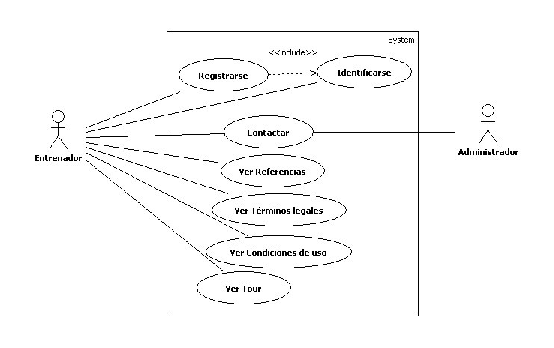
\includegraphics[width=15cm]{./eps/casos_uso/gestion_acceso.eps}
		  \caption{Paquete de gestión de acceso}
		  \label{fig:analisis_gestion_acceso}
		\end{figure}
		
	% subsection paquete_de_gestión_de_acceso (end)
	
	%
	%	Sub Paquete de Gestión de perfil
	%
	\subsection{Paquete de gestión de perfil} % (fold)
		\label{sub:paquete_de_gestion_de_perfil}
	
		El paquete de {\bf gestión de perfil} (figura \ref{fig:analisis_gestion_perfil}) contiene los casos de uso relacionados con el perfil y la sesión de un entrenador registrado. Cuando se ha identificado y accedido correctamente a la aplicación, un entrenador registrado puede ver y modificar sus datos personales introducidos en el proceso de registro. Además de ello, puede cambiar los datos de contacto y ajustar los parámetros del índice de Mujika según su forma de entrenar.
		
		Haciendo referencia a la sesión de un entrenador registrado se encuentran los casos de uso de cerrar sesión y de cambiar contraseña. 
		
		\begin{figure}[H]
		  \centering
		    \includegraphics[width=15.5cm]{./eps/casos_uso/gestion_perfil.eps}
		  \caption{Paquete de gestión del perfil}
		  \label{fig:analisis_gestion_perfil}
		\end{figure}
		
	% subsection paquete_de_gestión_de_perfil (end)
	
	%
	%	Sub Paquete de Gestión de nadadores
	%
	\subsection{Paquete de gestión de nadadores} % (fold)
		\label{sub:paquete_de_gestion_de_nadadores}
		
		El paquete de {\bf gestión de nadadores} (figura \ref{fig:analisis_gestion_nadadores}) es la base de la aplicación. Como se ha mencionado en otros capítulos, el recurso activo fundamental de todo entrenador es el nadador. Por ello, este conjunto de casos de uso representan las acciones que se pueden realizar respecto al control de los nadadores.
		
		Una de las tareas podría hacer un entrenador al acceder a la aplicación es añadir un nadador, con lo que se crearía una {\it ficha virtual}\footnote{Se traslada el concepto físico de ficha personal de un nadador al mundo virtual.} del mismo. En ella aparecerán los datos personales del nadador, y más adelante, cuando se añadan competiciones y test, se podrá visualizar la información de sus resultados.
		
		Así como se pueden añadir nadadores, el entrenador puede eliminarlos, modificarlos o verlos. Como en el resto de paquetes, estos casos de uso son denominados {\it CRUD} ({\it create, update and delete}). Hay dos corrientes en la creación efectiva de casos de uso: % mencionar fuentes
		
		\begin{itemize}
			\item {{\bf Abstraerlos y unirlos en un único caso de uso}. Lo que en casos podría beneficiar para disminuir el número de casos de uso en aplicaciones más grandes.}
			\item {{\bf Separarlos}. Si se desea tener un control mayor sobre cada caso de uso, más facilidad de reutilización y reducción de su complejidad.}
		\end{itemize}
		
		En este caso, se ha optado por dividirlos en distintos casos de uso, con lo que su especificación será más fácil y se podrán desarrollar en iteraciones diferentes.
		
		Una vez que se han añadido los nadadores, los entrenadores pueden ver una lista con ellos, mostrándose los datos más relevantes de los mismos. En caso de que se necesite realizar una búsqueda de los mismos, la aplicación permite esta funcionalidad tanto para realizar una búsqueda por nombre como por categoría.
		 
		\begin{figure}[H]
		  \centering
		    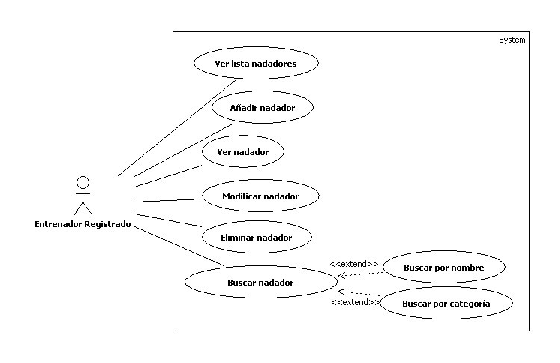
\includegraphics[width=15cm]{./eps/casos_uso/gestion_nadadores.eps}
		  \caption{Paquete de gestión de nadadores}
		  \label{fig:analisis_gestion_nadadores}
		\end{figure}
		
	% subsection paquete_de_gestión_de_nadadores (end)
	
	%
	%	Sub Paquete de Gestión de entrenamientos
	%
	\subsection{Paquete de gestión de entrenamientos} % (fold)
		\label{sub:paquete_de_gestion_de_entrenamientos}
		
		El paquete de {\bf gestión de entrenamientos} (figura \ref{fig:analisis_gestion_entrenamientos}) contiene los casos de uso relacionados con los entrenamientos diarios realizados por un entrenador registrado, donde el primero de los casos de uso que aparece es el de añadir planificación. En él se especifica que un entrenador tiene la posibilidad de adjuntar a la aplicación fichero con la planificación realizada para la temporada.
		
		A medida que se añaden, ven, modifican o eliminan entrenamientos, se va contemplando la carga de volumen e intensidad que desarrollan los nadadores en las sesiones. Una vez añadidos, el entrenador podrá ver una lista con ellos e incluso buscar alguno específicamente.
		
		Cada entrenamiento se compone de distintos ejercicios. Pues bien, los casos de uso de añadir, modificar y eliminar ejercicio cubren esa función. 
		
		\begin{figure}[H]
		  \centering
		    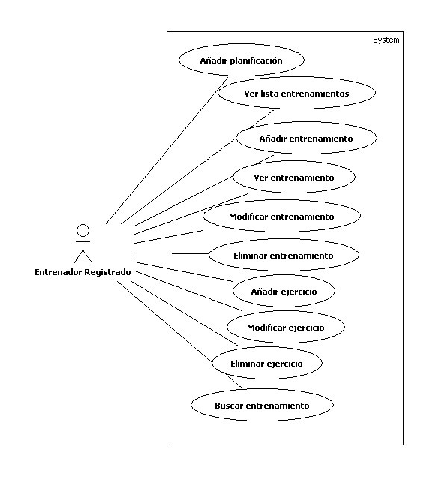
\includegraphics[width=13cm]{./eps/casos_uso/gestion_entrenamientos.eps}
		  \caption{Paquete de gestión de los entrenamientos}
		  \label{fig:analisis_gestion_entrenamientos}
		\end{figure}
	
	% subsection paquete_de_gestión_de_entrenamientos (end)

	%
	%	Sub Paquete de Gestión de competiciones
	%
	\subsection{Paquete de gestión de competiciones} % (fold)
		\label{sub:paquete_de_gestion_de_competiciones}
		
		El paquete de {\bf gestión de competiciones} (figura \ref{fig:analisis_gestion_competiciones}) contiene los casos de uso relacionados con las competiciones a las cuál asiste un entrenador o los nadadores del mismo. Un entrenador registrado puede añadir, ver, modificar o eliminar una competición. En ella se muestran los datos de donde se realiza, tipo de cronómetro, fecha o longitud de la piscina.
		
		A una competición existen asociados resultados de los nadadores que compiten. Estos resultados se registran con los casos de uso de añadir, modificar o eliminar resultado de nadador. Contienen la prueba que ha realizado el nadador y el tiempo obtenido (entre otros datos menos relevantes).
		
		Al igual que en los paquetes anteriores, aparece el poder buscar una competición o ver una lista con todas ellas. La diferencia radica en que el listado se puede ver como calendario.
		
		\begin{figure}[H]
		  \centering
		    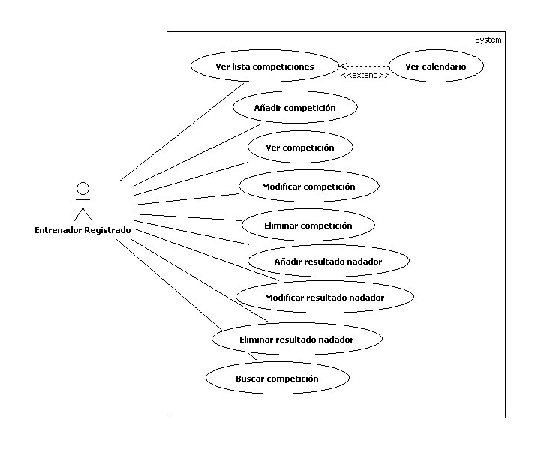
\includegraphics[width=15cm]{./eps/casos_uso/gestion_competiciones.eps}
		  \caption{Paquete de gestión de las competiciones}
		  \label{fig:analisis_gestion_competiciones}
		\end{figure}
		
	% subsection paquete_de_gestión_de_competiciones (end)
	
	%
	%	Sub Paquete de Gestión de test
	%
	
	\subsection{Paquete de gestión de test} % (fold)
		\label{sub:paquete_de_gestion_de_test}
		
		El paquete de {\bf gestión de test} (figura \ref{fig:analisis_gestion_test}) contiene los casos de uso relacionados con los test que realiza un entrenador y que registra los resultados de los nadadores. En ellos se miden tanto capacidades fisiológicas como deportivas \footnote{Entiéndase por capacidad fisiológica las que miden parámetros físicos y biológicos ---altura, peso, envergadura---; como capacidad deportiva las que realizan tomas de datos para comprobar la puesta a punto deportivamente ---test de velocidad o de resistencia.}.
		
		Por tanto, un entrenador registrado puede añadir, ver, modificar o eliminar un test. Nuevamente, al añadir se ingresan los datos de lugar, fecha y nombre del test. A raíz de ahí, se insertan los resultados que cada nadador ha obtenido en dicho test. Esto último se realiza con los casos de uso de añadir, eliminar o modificar resultados al test. 
		
		\begin{figure}[H]
		  \centering
		    \includegraphics[width=10cm]{./eps/casos_uso/gestion_test.eps}
		  \caption{Paquete de gestión de los test}
		  \label{fig:analisis_gestion_test}
		\end{figure}
	
	% subsection paquete_de_gestión_de_test (end)
	
	%
	%	Sub Paquete de Gestión de diario de incidencias
	%
	\subsection{Paquete de gestión de diario de incidencias} % (fold)
		\label{sub:paquete_de_gestion_de_diario_de_incidencias}
	
		El paquete de {\bf gestión de diario de incidencias} (figura \ref{fig:analisis_gestion_incidencias}) contiene los casos de uso relacionados con las incidencias con las que se encuentra un entrenador a lo largo de una temporada deportiva.
		
		Los casos de uso de añadir, ver, modificar o eliminar registro de incidencia, conforman la estructura del paquete. Con ellos, un entrenador añade incidencias al sistema en forma de diario. Posteriormente, el entrenador puede revisarlo o buscar entre todos los registros de incidencia el que requiera.
		
		\begin{figure}[H]
		  \centering
		    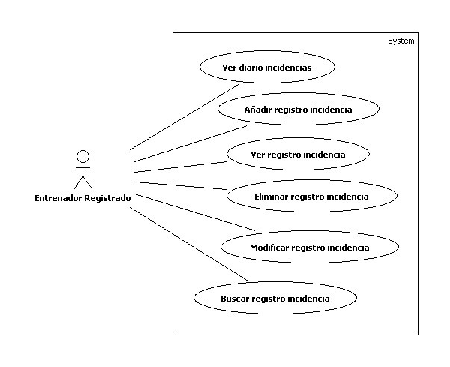
\includegraphics[width=13cm]{./eps/casos_uso/gestion_incidencias.eps}
		  \caption{Paquete de gestión de diario de incidencias}
		  \label{fig:analisis_gestion_incidencias}
		\end{figure}
		
	% subsection paquete_de_gestión_de_diario_de_incidencias (end)
	
	%
	%	Sub Paquete Imprimir
	%
	\subsection{Paquete imprimir} % (fold)
		\label{sub:paquete_imprimir}
		El paquete {\bf imprimir} (figura \ref{fig:analisis_imprimir}) contiene los casos de uso para la impresión de datos. Debido a que será un servicio de aplicación, se ha separado en un paquete a parte. En esta versión de la aplicación, únicamente se podrá imprimir la lista de nadadores.
		
		\begin{figure}[H]
		  \centering
		    \includegraphics[width=11.5cm]{./eps/casos_uso/imprimir.eps}
		  \caption{Paquete imprimir}
		  \label{fig:analisis_imprimir}
		\end{figure}
		
	% subsection paquete_imprimir (end)
	
	\newpage
	
	\subsection{Especificación de casos de uso} % (fold)
		\label{sub:especificacion_de_casos_de_uso}
		
		No hay duda de que el modo de especificación tiene mucho que ver con la calidad de la solución. Los ingenieros del software que se han visto forzados a trabajar con especificaciones incompletas, inconsistentes o engañosas han experimentado la frustración y confusión que invariablemente provocan. La calidad, la fecha de entrega y el alcance del software son las que sufren las consecuencias.
		
		La especificación, independientemente del modo como la realicemos, puede verse como un proceso de representación. Los requisitos se representan de manera que como fin último lleven al éxito de la implementación del software. A continuación, se proponen algunos principios de especificación adaptados del trabajo de Balzer y Goldman \cite{BAL86}:
		
		\begin{enumerate}
			\item {Separar la funcionalidad de la implementación.}
			\item {Desarrollar un modelo del comportamiento deseado de un sistema que comprenda datos y las respuestas funcionales de un sistema a varios estímulos del entorno.}
			\item {Establecer el contexto en que opera el software especificando la manera en que otros componentes del sistema interactúan con él.}
			\item {Definir el entorno en que va a operar el sistema e indicar como una <<colección de agentes altamente entrelazados reaccionan a estímulos del entornos (cambios de objetos) producidos por esos agentes>>.}
			\item {Crear un modelo intuitivo en vez de un diseño o modelo de implementación.}
			\item {Reconocer que la <<especificación debe ser tolerante a un posible crecimiento si no es completa>>. Una especificación es siempre un modelo ---una abstracción--- de alguna situación real (o prevista) que normalmente suele ser compleja. De ahí, que será incompleta y existirá a muchos niveles de detalle.}
			\item {Establecer el contenido y la estructura de una especificación de manera que acepte cambios.}
		\end{enumerate}
		
		Esta lista de principios básicos proporciona la base para representar los requisitos del software. Sin embargo, los principios deben traducirse en realidad. Por ello, en a continuación se muestran las especificaciones de los casos de uso detectados en el modelo.
		
		% ------------- Caso de uso [Gestión Acceso] Registrarse
		\begin{table}[H]
		\begin{tabular}{|p{12cm}|p{12cm}|p{12cm}|} 
			\hline 
				\multicolumn{3}{|l|}{{\bf Especificación de Caso de Uso: Registrarse}}\\ 
			\hline
				\multicolumn{2}{|l|}{{\bf ID}} & ECU-PGA.01\\ 
			\hline 
				\multicolumn{2}{|l|}{{\bf Nombre}} & Registrarse\\ 
			\hline
				\multicolumn{2}{|l|}{{\bf Descripción}} & Realiza el registro en la aplicación de un entrenador aún no registrado\\ 
			\hline
				\multicolumn{2}{|l|}{{\bf Actores}} & Entrenador\\ 
			\hline
				\multicolumn{2}{|l|}{{\bf Precondiciones}} & ---\\ 
			\hline
				\multicolumn{2}{|l|}{{\bf Postcondiciones}} & Se registra en el sistema al entrenador\\
					%El entrenador pasa a ser entrenador registrado, con lo que puede acceder al sistema\\ 
			\hline
				\multicolumn{3}{|l|}{{\bf Flujo Normal de Eventos}}\\ 			
			\hline
				\multicolumn{3}{|l|}{
					{\begin{tabular}{lp{14cm}}					
						1. & El entrenador selecciona la opción de registrarse\\ 
						2. & El sistema muestra un formulario de registro con los campos de: {\it nombre, apellidos, email, contraseña y confirmar contraseña}\\ 
						3. & El entrenador rellena cada campo del formulario y pulsa el botón de enviar\\
						4. & El sistema valida los datos del formulario y registra al entrenador
					\end{tabular}}}\\
			\hline
				\multicolumn{3}{|l|}{{\bf Flujos Alternativos}}\\ 
			\hline
				\multicolumn{3}{|l|}{
					{\begin{tabular}{lp{14cm}}					
						3.1. & Si el entrenador no rellena todos los campos del formulario, el sistema muestra un error y vuelve al paso 2\\
						3.2. & Si la contraseña insertada no es igual a la confirmación de contraseña, el sistema muestra un error y vuelve al paso 2\\ 
						4.1. & Si el sistema encuentra error en la validación de datos del formulario, muestra mensaje de error y vuelve al paso 2 
					\end{tabular}}}\\
			\hline
		\end{tabular}
		\caption{Especificación caso de uso registrarse}
		\end{table} 
		
		% ------------- Caso de uso [Gestión Acceso] Identificarse
		\begin{table}[H]
		\begin{tabular}{|p{12cm}|p{12cm}|p{12cm}|} 
			\hline 
				\multicolumn{3}{|l|}{{\bf Especificación de Caso de Uso: Identificarse}}\\ 
			\hline
				\multicolumn{2}{|l|}{{\bf ID}} & ECU-PGA.02\\ 
			\hline 
				\multicolumn{2}{|l|}{{\bf Nombre}} & Identificarse\\ 
			\hline
				\multicolumn{2}{|l|}{{\bf Descripción}} & Permite el acceso a un entrenador a la aplicación\\ 
			\hline
				\multicolumn{2}{|l|}{{\bf Actores}} & Entrenador\\ 
			\hline
				\multicolumn{2}{|l|}{{\bf Precondiciones}} & Entrenador tiene que estar registrado en el sistema\\ 
			\hline
				\multicolumn{2}{|l|}{{\bf Postcondiciones}} & Entrenador accede al sistema \\ 
			\hline
				\multicolumn{3}{|l|}{{\bf Flujo Normal de Eventos}}\\ 			
			\hline
				\multicolumn{3}{|l|}{
					{\begin{tabular}{lp{14cm}}
						%\multicolumn{2}{l}{Cancelar ejecución}\\
						1. & El entrenador selecciona la opción de identificarse\\
						2. & El sistema muestra un formulario con los campos de identificación: {\it email y contraseña}\\
						3. & El entrenador rellena los campos del formulario de identificación y pulsa el botón de enviar\\
						4. & El sistema valida los datos del formulario\\
						5. & El sistema inicia una sesión en la aplicación para el entrenador identificado\\
						6. & El sistema muestra la página de resumen del entrenador identificado					
					\end{tabular}}}\\
			\hline
				\multicolumn{3}{|l|}{{\bf Flujos Alternativos}}\\ 
			\hline
				\multicolumn{3}{|l|}{
					{\begin{tabular}{lp{14cm}} 
						3.1. & Si el entrenador no rellena todos los campos del formulario, el sistema envía un mensaje de error y vuelve al paso 2\\
						4.1. & Si los datos de identificación no coinciden con el email y la contraseña de un entrenador registrado, el sistema muestra un mensaje de error y vuelve al paso 2						
					\end{tabular}}}\\
			\hline
		\end{tabular}
		\caption{Especificación caso de uso identificarse}
		\end{table}
		
		% ------------- Caso de uso [Gestión Acceso] Contactar
		\begin{table}[H]
		\begin{tabular}{|p{12cm}|p{12cm}|p{12cm}|} 
			\hline 
				\multicolumn{3}{|l|}{{\bf Especificación de Caso de Uso: Contactar}}\\ 
			\hline
				\multicolumn{2}{|l|}{{\bf ID}} & ECU-PGA.03\\ 
			\hline 
				\multicolumn{2}{|l|}{{\bf Nombre}} & Contactar\\ 
			\hline
				\multicolumn{2}{|l|}{{\bf Descripción}} & Permite realizar la puesta en contacto de un entrenador con un administrador\\ 
			\hline
				\multicolumn{2}{|l|}{{\bf Actores}} & Entrenador, administrador\\ 
			\hline
				\multicolumn{2}{|l|}{{\bf Precondiciones}} & ---\\ 
			\hline
				\multicolumn{2}{|l|}{{\bf Postcondiciones}} & Mensaje de entrenador entregado al administrador\\ 
			\hline
				\multicolumn{3}{|l|}{{\bf Flujo Normal de Eventos}}\\ 			
			\hline
				\multicolumn{3}{|l|}{
					{\begin{tabular}{lp{14cm}} 
						1. & El entrenador selecciona la opción de contactar con administrador\\
						2. & El sistema muestra una página estática con la información de contacto y con un formulario con los campos de: {\it nombre, email, titulo, mensaje}\\
						3. & El entrenador rellena los campos del formulario y pulsa el botón de enviar\\
						4. & El sistema comprueba que se hayan rellenado todos los datos y envía la información al email de contacto del administrador						
					\end{tabular}}}\\
			\hline
				\multicolumn{3}{|l|}{{\bf Flujos Alternativos}}\\ 
			\hline
				\multicolumn{3}{|l|}{
					{\begin{tabular}{lp{14cm}} 
						4.1. & Si el sistema detecta que no se han rellenado todos los campos del formulario, muestra un mensaje de error y vuelve al paso 2\\
						4.2. & Si el sistema detecta que el email no tiene una estructura correcta, muestra un mensaje de error y vuelve al paso 2
					\end{tabular}}}\\
			\hline
		\end{tabular}
		\caption{Especificación caso de uso contactar}
		\end{table}
		
		% ------------- Caso de uso [Gestión Acceso] Ver Referencias
		\begin{table}[H]
		\begin{tabular}{|p{12cm}|p{12cm}|p{12cm}|} 
			\hline 
				\multicolumn{3}{|l|}{{\bf Especificación de Caso de Uso: Ver referencias}}\\ 
			\hline
				\multicolumn{2}{|l|}{{\bf ID}} & ECU-PGA.04\\ 
			\hline 
				\multicolumn{2}{|l|}{{\bf Nombre}} & Ver referencias\\ 
			\hline
				\multicolumn{2}{|l|}{{\bf Descripción}} & Muestra una página estática con las referencias realizadas por los entrenadores que han intervenido en el proceso de creación de la aplicación\\ 
			\hline
				\multicolumn{2}{|l|}{{\bf Actores}} & Entrenador\\ 
			\hline
				\multicolumn{2}{|l|}{{\bf Precondiciones}} & ---\\ 
			\hline
				\multicolumn{2}{|l|}{{\bf Postcondiciones}} & Entrenador ve las referencias de la aplicación\\ 
			\hline
				\multicolumn{3}{|l|}{{\bf Flujo Normal de Eventos}}\\ 			
			\hline
				\multicolumn{3}{|l|}{
					{\begin{tabular}{lp{14cm}} 
						1. & El entrenador selecciona la opción de ver referencias de la aplicación\\
						2. & El sistema muestra una página estática con toda la información acerca de las referencias de la aplicación						
					\end{tabular}}}\\
			\hline
				\multicolumn{3}{|l|}{{\bf Flujos Alternativos}}\\ 
			\hline
				\multicolumn{3}{|l|}{
					{\begin{tabular}{lp{14cm}} 
						---
					\end{tabular}}}\\
			\hline
		\end{tabular}
		\caption{Especificación caso de uso ver referencias}
		\end{table}
		
		% ------------- Caso de uso [Gestión Acceso] Ver Términos Legales
		\begin{table}[H]
		\begin{tabular}{|p{12cm}|p{12cm}|p{12cm}|} 
			\hline 
				\multicolumn{3}{|l|}{{\bf Especificación de Caso de Uso: Ver términos legales}}\\ 
			\hline
				\multicolumn{2}{|l|}{{\bf ID}} & ECU-PGA.05\\ 
			\hline 
				\multicolumn{2}{|l|}{{\bf Nombre}} & Ver términos legales\\ 
			\hline
				\multicolumn{2}{|l|}{{\bf Descripción}} & Muestra una página estática con los términos legales de la aplicación\\ 
			\hline
				\multicolumn{2}{|l|}{{\bf Actores}} & Entrenador\\ 
			\hline
				\multicolumn{2}{|l|}{{\bf Precondiciones}} & ---\\ 
			\hline
				\multicolumn{2}{|l|}{{\bf Postcondiciones}} & Entrenador ve los términos legales de la aplicación\\ 
			\hline
				\multicolumn{3}{|l|}{{\bf Flujo Normal de Eventos}}\\ 			
			\hline
				\multicolumn{3}{|l|}{
					{\begin{tabular}{lp{14cm}} 
						1. & El entrenador selecciona la opción de ver términos legales del a aplicación\\
						2. & El sistema muestra una página estática con toda la información acerca de los términos legales de la aplicación
					\end{tabular}}}\\
			\hline
				\multicolumn{3}{|l|}{{\bf Flujos Alternativos}}\\ 
			\hline
				\multicolumn{3}{|l|}{
					{\begin{tabular}{lp{14cm}} 
						---						
					\end{tabular}}}\\
			\hline
		\end{tabular}
		\caption{Especificación caso de uso ver términos legales}
		\end{table}
		
		% ------------- Caso de uso [Gestión Acceso] Ver Condiciones de Uso
		\begin{table}[H]
		\begin{tabular}{|p{12cm}|p{12cm}|p{12cm}|} 
			\hline 
				\multicolumn{3}{|l|}{{\bf Especificación de Caso de Uso: Ver condiciones de uso}}\\ 
			\hline
				\multicolumn{2}{|l|}{{\bf ID}} & ECU-PGA.06\\ 
			\hline 
				\multicolumn{2}{|l|}{{\bf Nombre}} & Ver condiciones de uso\\ 
			\hline
				\multicolumn{2}{|l|}{{\bf Descripción}} & Muestra una página estática con las condiciones de uso de la aplicación\\ 
			\hline
				\multicolumn{2}{|l|}{{\bf Actores}} & Entrenador\\ 
			\hline
				\multicolumn{2}{|l|}{{\bf Precondiciones}} & ---\\ 
			\hline
				\multicolumn{2}{|l|}{{\bf Postcondiciones}} & Entrenador ve las condiciones de uso de la aplicación\\ 
			\hline
				\multicolumn{3}{|l|}{{\bf Flujo Normal de Eventos}}\\ 			
			\hline
				\multicolumn{3}{|l|}{
					{\begin{tabular}{lp{14cm}} 
						1. & El entrenador selecciona la opción de ver condiciones de uso de la aplicación\\
						2. & El sistema muestra una página estática con toda la información acerca de las condiciones de uso de la aplicación
					\end{tabular}}}\\
			\hline
				\multicolumn{3}{|l|}{{\bf Flujos Alternativos}}\\ 
			\hline
				\multicolumn{3}{|l|}{
					{\begin{tabular}{lp{14cm}} 
						---
					\end{tabular}}}\\
			\hline
		\end{tabular}
		\caption{Especificación caso de uso ver condiciones de uso}
		\end{table}
		
		% ------------- Caso de uso [Gestión Acceso] Ver Tour
		\begin{table}[H]
		\begin{tabular}{|p{12cm}|p{12cm}|p{12cm}|} 
			\hline 
				\multicolumn{3}{|l|}{{\bf Especificación de Caso de Uso: Ver tour}}\\ 
			\hline
				\multicolumn{2}{|l|}{{\bf ID}} & ECU-PGA.07\\ 
			\hline 
				\multicolumn{2}{|l|}{{\bf Nombre}} & Ver tour\\ 
			\hline
				\multicolumn{2}{|l|}{{\bf Descripción}} & Muestra una página estática como interfaz de entrada, con un tour de las características de la aplicación\\ 
			\hline
				\multicolumn{2}{|l|}{{\bf Actores}} & Entrenador\\ 
			\hline
				\multicolumn{2}{|l|}{{\bf Precondiciones}} & ---\\ 
			\hline
				\multicolumn{2}{|l|}{{\bf Postcondiciones}} & Entrenador ve el tour de la aplicación\\ 
			\hline
				\multicolumn{3}{|l|}{{\bf Flujo Normal de Eventos}}\\ 			
			\hline
				\multicolumn{3}{|l|}{
					{\begin{tabular}{lp{14cm}} 
						1. & El entrenador selecciona la opción de ver tour de la aplicación\\
						2. & El sistema muestra una página estática con toda la información acerca del tour de la aplicación
					\end{tabular}}}\\
			\hline
				\multicolumn{3}{|l|}{{\bf Flujos Alternativos}}\\ 
			\hline
				\multicolumn{3}{|l|}{
					{\begin{tabular}{lp{14cm}} 
						---
					\end{tabular}}}\\
			\hline
		\end{tabular}
		\caption{Especificación caso de uso ver tour}
		\end{table}
		
		% ------------- Caso de uso [Gestión Perfil] Cerrar Sesión
		\begin{table}[H]
		\begin{tabular}{|p{12cm}|p{12cm}|p{12cm}|} 
			\hline 
				\multicolumn{3}{|l|}{{\bf Especificación de Caso de Uso: Cerrar sesión}}\\ 
			\hline
				\multicolumn{2}{|l|}{{\bf ID}} & ECU-PGP.01\\ 
			\hline 
				\multicolumn{2}{|l|}{{\bf Nombre}} & Cerrar sesión\\ 
			\hline
				\multicolumn{2}{|l|}{{\bf Descripción}} & Finaliza la sesión iniciada tras identificarse un entrenador registrado en el sistema\\ 
			\hline
				\multicolumn{2}{|l|}{{\bf Actores}} & Entrenador registrado\\ 
			\hline
				\multicolumn{2}{|l|}{{\bf Precondiciones}} & Entrenador registrado identificado\\ 
			\hline
				\multicolumn{2}{|l|}{{\bf Postcondiciones}} & Sistema finaliza la sesión del entrenador\\ 
			\hline
				\multicolumn{3}{|l|}{{\bf Flujo Normal de Eventos}}\\ 			
			\hline
				\multicolumn{3}{|l|}{
					{\begin{tabular}{lp{14cm}} 
						1. & El entrenador selecciona la opción de cerrar sesión\\
						2. & El sistema elimina la sesión iniciada por el entrenador\\
						3. & El sistema redirecciona al entrenador a la página principal de la aplicación
					\end{tabular}}}\\
			\hline
				\multicolumn{3}{|l|}{{\bf Flujos Alternativos}}\\ 
			\hline
				\multicolumn{3}{|l|}{
					{\begin{tabular}{lp{14cm}} 
						---
					\end{tabular}}}\\
			\hline
		\end{tabular}
		\caption{Especificación caso de uso cerrar sesión}
		\end{table}
		
		% ------------- Caso de uso [Gestión Perfil] Modificar perfil
		\begin{table}[H]
		\begin{tabular}{|p{12cm}|p{12cm}|p{12cm}|} 
			\hline 
				\multicolumn{3}{|l|}{{\bf Especificación de Caso de Uso: Modificar perfil}}\\ 
			\hline
				\multicolumn{2}{|l|}{{\bf ID}} & ECU-PGP.02\\ 
			\hline 
				\multicolumn{2}{|l|}{{\bf Nombre}} & Modificar perfil\\ 
			\hline
				\multicolumn{2}{|l|}{{\bf Descripción}} & Permite modificar el perfil de un entrenador registrado\\ 
			\hline
				\multicolumn{2}{|l|}{{\bf Actores}} & Entrenador registrado\\ 
			\hline
				\multicolumn{2}{|l|}{{\bf Precondiciones}} & ---\\ 
			\hline
				\multicolumn{2}{|l|}{{\bf Postcondiciones}} & ---\\ 
			\hline
				\multicolumn{3}{|l|}{{\bf Flujo Normal de Eventos}}\\ 			
			\hline
				\multicolumn{3}{|l|}{
					{\begin{tabular}{lp{14cm}} 
						---
						%\multicolumn{2}{l}{Cancelar ejecución}\\
						%1. & item dos\\ 
						%2. & subitem dos uno\\ 
						%2. & subitem dos dos
					\end{tabular}}}\\
			\hline
				\multicolumn{3}{|l|}{{\bf Flujos Alternativos}}\\ 
			\hline
				\multicolumn{3}{|l|}{
					{\begin{tabular}{lp{14cm}} 
						---
						%\multicolumn{2}{l}{Cancelar ejecución}\\
						%1. & item dos\\ 
						%2. & subitem dos uno\\ 
						%2. & subitem dos dos
					\end{tabular}}}\\
			\hline
		\end{tabular}
		\caption{Especificación caso de uso modificar perfil}
		\end{table}
		
		% ------------- Caso de uso [Gestión Perfil] Modificar datos personales
		\begin{table}[H]
		\begin{tabular}{|p{12cm}|p{12cm}|p{12cm}|} 
			\hline 
				\multicolumn{3}{|l|}{{\bf Especificación de Caso de Uso: Modificar datos personales}}\\ 
			\hline
				\multicolumn{2}{|l|}{{\bf ID}} & ECU-PGP.03\\ 
			\hline 
				\multicolumn{2}{|l|}{{\bf Nombre}} & Modificar datos personales\\ 
			\hline
				\multicolumn{2}{|l|}{{\bf Descripción}} & Un entrenador registrado debe poder modificar los datos personales asociados al mismo\\ 
			\hline
				\multicolumn{2}{|l|}{{\bf Actores}} & Entrenador registrado\\ 
			\hline
				\multicolumn{2}{|l|}{{\bf Precondiciones}} & ---\\ 
			\hline
				\multicolumn{2}{|l|}{{\bf Postcondiciones}} & ---\\ 
			\hline
				\multicolumn{3}{|l|}{{\bf Flujo Normal de Eventos}}\\ 			
			\hline
				\multicolumn{3}{|l|}{
					{\begin{tabular}{lp{14cm}} 
						---
						%\multicolumn{2}{l}{Cancelar ejecución}\\
						%1. & item dos\\ 
						%2. & subitem dos uno\\ 
						%2. & subitem dos dos
					\end{tabular}}}\\
			\hline
				\multicolumn{3}{|l|}{{\bf Flujos Alternativos}}\\ 
			\hline
				\multicolumn{3}{|l|}{
					{\begin{tabular}{lp{14cm}} 
						---
						%\multicolumn{2}{l}{Cancelar ejecución}\\
						%1. & item dos\\ 
						%2. & subitem dos uno\\ 
						%2. & subitem dos dos
					\end{tabular}}}\\
			\hline
		\end{tabular}
		\caption{Especificación caso de uso modificar datos personales}
		\end{table}
		
		% ------------- Caso de uso [Gestión Perfil] Modificar datos de contacto
		\begin{table}[H]
		\begin{tabular}{|p{12cm}|p{12cm}|p{12cm}|} 
			\hline 
				\multicolumn{3}{|l|}{{\bf Especificación de Caso de Uso: Modificar datos de contacto}}\\ 
			\hline
				\multicolumn{2}{|l|}{{\bf ID}} & ECU-PGP.04\\ 
			\hline 
				\multicolumn{2}{|l|}{{\bf Nombre}} & Modificar datos de contacto\\ 
			\hline
				\multicolumn{2}{|l|}{{\bf Descripción}} & Un entrenador registrado debe poder modificar los datos de contacto asociados al mismo\\ 
			\hline
				\multicolumn{2}{|l|}{{\bf Actores}} & Entrenador registrado\\ 
			\hline
				\multicolumn{2}{|l|}{{\bf Precondiciones}} & ---\\ 
			\hline
				\multicolumn{2}{|l|}{{\bf Postcondiciones}} & ---\\ 
			\hline
				\multicolumn{3}{|l|}{{\bf Flujo Normal de Eventos}}\\ 			
			\hline
				\multicolumn{3}{|l|}{
					{\begin{tabular}{lp{14cm}} 
						---
						%\multicolumn{2}{l}{Cancelar ejecución}\\
						%1. & item dos\\ 
						%2. & subitem dos uno\\ 
						%2. & subitem dos dos
					\end{tabular}}}\\
			\hline
				\multicolumn{3}{|l|}{{\bf Flujos Alternativos}}\\ 
			\hline
				\multicolumn{3}{|l|}{
					{\begin{tabular}{lp{14cm}} 
						---
						%\multicolumn{2}{l}{Cancelar ejecución}\\
						%1. & item dos\\ 
						%2. & subitem dos uno\\ 
						%2. & subitem dos dos
					\end{tabular}}}\\
			\hline
		\end{tabular}
		\caption{Especificación caso de uso modificar datos de contacto}
		\end{table}
		
		% ------------- Caso de uso [Gestión Perfil] Modificar índice de Mujika
		\begin{table}[H]
		\begin{tabular}{|p{12cm}|p{12cm}|p{12cm}|} 
			\hline 
				\multicolumn{3}{|l|}{{\bf Especificación de Caso de Uso: Modificar índice de Mujika}}\\ 
			\hline
				\multicolumn{2}{|l|}{{\bf ID}} & ECU-PGP.05\\ 
			\hline 
				\multicolumn{2}{|l|}{{\bf Nombre}} & Modificar índice de Mujika\\ 
			\hline
				\multicolumn{2}{|l|}{{\bf Descripción}} & Un entenador registrado debe poder modificar los valores del parámetro del índice de Mujika\\ 
			\hline
				\multicolumn{2}{|l|}{{\bf Actores}} & Entrenador registrado\\ 
			\hline
				\multicolumn{2}{|l|}{{\bf Precondiciones}} & ---\\ 
			\hline
				\multicolumn{2}{|l|}{{\bf Postcondiciones}} & ---\\ 
			\hline
				\multicolumn{3}{|l|}{{\bf Flujo Normal de Eventos}}\\ 			
			\hline
				\multicolumn{3}{|l|}{
					{\begin{tabular}{lp{14cm}} 
						---
						%\multicolumn{2}{l}{Cancelar ejecución}\\
						%1. & item dos\\ 
						%2. & subitem dos uno\\ 
						%2. & subitem dos dos
					\end{tabular}}}\\
			\hline
				\multicolumn{3}{|l|}{{\bf Flujos Alternativos}}\\ 
			\hline
				\multicolumn{3}{|l|}{
					{\begin{tabular}{lp{14cm}} 
						---
						%\multicolumn{2}{l}{Cancelar ejecución}\\
						%1. & item dos\\ 
						%2. & subitem dos uno\\ 
						%2. & subitem dos dos
					\end{tabular}}}\\
			\hline
		\end{tabular}
		\caption{Especificación caso de uso modificar índice de Mujika}
		\end{table}
		
		% ------------- Caso de uso [Gestión Perfil] Ver perfil
		\begin{table}[H]
		\begin{tabular}{|p{12cm}|p{12cm}|p{12cm}|} 
			\hline 
				\multicolumn{3}{|l|}{{\bf Especificación de Caso de Uso: Ver perfil}}\\ 
			\hline
				\multicolumn{2}{|l|}{{\bf ID}} & ECU-PGP.06\\ 
			\hline 
				\multicolumn{2}{|l|}{{\bf Nombre}} & Modificar perfil\\ 
			\hline
				\multicolumn{2}{|l|}{{\bf Descripción}} & Muestra el perfil del entrenador registrado. Incluye tanto los datos personales como los datos de contacto\\ 
			\hline
				\multicolumn{2}{|l|}{{\bf Actores}} & Entrenador registrado\\ 
			\hline
				\multicolumn{2}{|l|}{{\bf Precondiciones}} & Entrenador identificado en la aplicación\\ 
			\hline
				\multicolumn{2}{|l|}{{\bf Postcondiciones}} & Entrenador ve el perfil\\ 
			\hline
				\multicolumn{3}{|l|}{{\bf Flujo Normal de Eventos}}\\ 			
			\hline
				\multicolumn{3}{|l|}{
					{\begin{tabular}{lp{14cm}} 
						1. & El entrenador selecciona la opción de ver perfil\\
						2. & El sistema muestra los datos del perfil del entrenador registrado\\
					\end{tabular}}}\\
			\hline
				\multicolumn{3}{|l|}{{\bf Flujos Alternativos}}\\ 
			\hline
				\multicolumn{3}{|l|}{
					{\begin{tabular}{lp{14cm}} 
						---
					\end{tabular}}}\\
			\hline
		\end{tabular}
		\caption{Especificación caso de uso modificar perfil}
		\end{table}
		
		% ------------- Caso de uso [Gestión Perfil] Cambiar contraseña
		\begin{table}[H]
		\begin{tabular}{|p{12cm}|p{12cm}|p{12cm}|} 
			\hline 
				\multicolumn{3}{|l|}{{\bf Especificación de Caso de Uso: Cambiar contraseña}}\\ 
			\hline
				\multicolumn{2}{|l|}{{\bf ID}} & ECU-PGP.07\\ 
			\hline 
				\multicolumn{2}{|l|}{{\bf Nombre}} & Cambiar contraseña\\ 
			\hline
				\multicolumn{2}{|l|}{{\bf Descripción}} & Permite que un entrenador registrado cambie la contraseña de acceso a la aplicación\\ 
			\hline
				\multicolumn{2}{|l|}{{\bf Actores}} & Entrenador registrado\\ 
			\hline
				\multicolumn{2}{|l|}{{\bf Precondiciones}} & Entrenador está identificado y viendo su perfil\\ 
			\hline
				\multicolumn{2}{|l|}{{\bf Postcondiciones}} & Actualizada la contraseña del entrenador registrado\\ 
			\hline
				\multicolumn{3}{|l|}{{\bf Flujo Normal de Eventos}}\\ 			
			\hline
				\multicolumn{3}{|l|}{
					{\begin{tabular}{lp{14cm}} 
						1. & El entrenador selecciona la opción cambiar contraseña\\
						2. & El sistema muestra un formulario con los campos de: {\it contraseña actual, nueva contraseña y confirmar nueva contraseña}\\
						3. & El entrenador inserta en el formulario los valores de cada uno de los campos\\
						4. & El sistema comprueba que la contraseña actual sea la correcta. Posteriormente, actualiza los valores de la nueva contraseña y muestra un mensaje de contraseña modificada correctamente						
					\end{tabular}}}\\
			\hline
				\multicolumn{3}{|l|}{{\bf Flujos Alternativos}}\\ 
			\hline
				\multicolumn{3}{|l|}{
					{\begin{tabular}{lp{14cm}} 
						4.1. & Si la contraseña actual no es correcta, el sistema muestra un mensaje de error y vuelve al paso 2
					\end{tabular}}}\\
			\hline
		\end{tabular}
		\caption{Especificación caso de uso cambiar contraseña}
		\end{table}
		
		% ------------- Caso de uso [Gestión Nadadores] Ver lista nadadores
		\begin{table}[H]
		\begin{tabular}{|p{12cm}|p{12cm}|p{12cm}|} 
			\hline 
				\multicolumn{3}{|l|}{{\bf Especificación de Caso de Uso: Ver lista nadadores}}\\ 
			\hline
				\multicolumn{2}{|l|}{{\bf ID}} & ECU-PGN.01\\ 
			\hline 
				\multicolumn{2}{|l|}{{\bf Nombre}} & Ver lista nadadores\\ 
			\hline
				\multicolumn{2}{|l|}{{\bf Descripción}} & Muestra el listado de nadadores insertados por un entrenador en la aplicación\\ 
			\hline
				\multicolumn{2}{|l|}{{\bf Actores}} & Entrenador registrado\\ 
			\hline
				\multicolumn{2}{|l|}{{\bf Precondiciones}} & Entrenador identificado en la aplicación\\ 
			\hline
				\multicolumn{2}{|l|}{{\bf Postcondiciones}} & ---\\ 
			\hline
				\multicolumn{3}{|l|}{{\bf Flujo Normal de Eventos}}\\ 			
			\hline
				\multicolumn{3}{|l|}{
					{\begin{tabular}{lp{14cm}} 
						1. & El entrenador selecciona la opción de ver lista de nadadores\\
						2. & El sistema muestra el listado de todos los nadadores pertenecientes al entrenador registrado
					\end{tabular}}}\\
			\hline
				\multicolumn{3}{|l|}{{\bf Flujos Alternativos}}\\ 
			\hline
				\multicolumn{3}{|l|}{
					{\begin{tabular}{lp{14cm}} 
						2.1 & Si el entrenador no ha insertado ningún nadador en el sistema, el sistema muestra un listado vacío con el comentario: <<no hay ningún nadador>>
					\end{tabular}}}\\
			\hline
		\end{tabular}
		\caption{Especificación caso de uso ver lista nadadores}
		\end{table}
		
		% ------------- Caso de uso [Gestión Nadadores] Añadir nadador
		\begin{table}[H]
		\begin{tabular}{|p{12cm}|p{12cm}|p{12cm}|} 
			\hline 
				\multicolumn{3}{|l|}{{\bf Especificación de Caso de Uso: Añadir nadador}}\\ 
			\hline
				\multicolumn{2}{|l|}{{\bf ID}} & ECU-PGN.02\\ 
			\hline 
				\multicolumn{2}{|l|}{{\bf Nombre}} & Añadir nadador\\ 
			\hline
				\multicolumn{2}{|l|}{{\bf Descripción}} & Permite a un entrenador registrado insertar un nadador en el sistema\\ 
			\hline
				\multicolumn{2}{|l|}{{\bf Actores}} & Entrenador registrado\\ 
			\hline
				\multicolumn{2}{|l|}{{\bf Precondiciones}} & Entrenador identificado en la aplicación\\ 
			\hline
				\multicolumn{2}{|l|}{{\bf Postcondiciones}} & Actualizada la lista de nadadores asociados al entrenador registrado\\ 
			\hline
				\multicolumn{3}{|l|}{{\bf Flujo Normal de Eventos}}\\ 			
			\hline
				\multicolumn{3}{|l|}{
					{\begin{tabular}{lp{14cm}} 
						1. & El entrenador selecciona la opción de añadir nadador\\
						2. & El sistema muestra un formulario con los campos: {\it nombre, apellidos, licencia, fecha de nacimiento, datos de contacto y observaciones}\\
						3. & El entrenador inserta los valores con los datos del nadador en cada uno de los campos y pulsa el botón de añadir\\
						4. & El sistema valida los campos y comprueba que los campos obligatorios estén cumplimentados\\
						5. & El sistema calcula la categoría del nadador en base a la fecha de nacimiento insertada\\
						6. & El sistema almacena el registro del nuevo nadador y muestra mensaje de nadador añadido correctamente
					\end{tabular}}}\\
			\hline
				\multicolumn{3}{|l|}{{\bf Flujos Alternativos}}\\ 
			\hline
				\multicolumn{3}{|l|}{
					{\begin{tabular}{lp{14cm}} 
						3.1. & Si el entrenador pulsa el botón de cancelar, ir a paso 3.2\\
						3.2. & El sistema no almacena el registro del nadador y cancela todo el proceso\\
						4.1. & Si el sistema detecta que no se han rellenado los campos obligatorios o hay fallo de validación de datos, el sistema muestra un mensaje de error y vuelve al paso 2\\
						4.2. & Si el valor de la fecha de nacimiento es posterior a fecha actual, el sistema muestra mensaje de error y vuelve al paso 2\\
						4.3. & Si existe un nadador perteneciente al entrenador con el mismo número de licencia, el sistema muestra un error y vuelve al paso 2\\
					\end{tabular}}}\\
			\hline
		\end{tabular}
		\caption{Especificación caso de uso añadir nadador}
		\end{table}
		
		% ------------- Caso de uso [Gestión Nadadores] Ver nadador
		\begin{table}[H]
		\begin{tabular}{|p{12cm}|p{12cm}|p{12cm}|} 
			\hline 
				\multicolumn{3}{|l|}{{\bf Especificación de Caso de Uso: Ver nadador}}\\ 
			\hline
				\multicolumn{2}{|l|}{{\bf ID}} & ECU-PGN.03\\ 
			\hline 
				\multicolumn{2}{|l|}{{\bf Nombre}} & Ver nadador\\ 
			\hline
				\multicolumn{2}{|l|}{{\bf Descripción}} & Muestra un nadador específico perteneciente al entrenador registrado\\ 
			\hline
				\multicolumn{2}{|l|}{{\bf Actores}} & Entrenador registrado\\ 
			\hline
				\multicolumn{2}{|l|}{{\bf Precondiciones}} & Entrenador está identificado y viendo el listado de nadadores\\ 
			\hline
				\multicolumn{2}{|l|}{{\bf Postcondiciones}} & ---\\ 
			\hline
				\multicolumn{3}{|l|}{{\bf Flujo Normal de Eventos}}\\ 			
			\hline
				\multicolumn{3}{|l|}{
					{\begin{tabular}{lp{14cm}} 
						1. & El entrenador selecciona el nadador que quiere ver de la lista de nadadores\\
						2. & El sistema muestra los datos pertenecientes al nadador especificado\\
						3. & El sistema muestra los resultados de las competiciones asociados al nadador seleccionado\\
						4. & El sistema muestra los resultados de los test realizados por el nadador seleccionado
					\end{tabular}}}\\
			\hline
				\multicolumn{3}{|l|}{{\bf Flujos Alternativos}}\\ 
			\hline
				\multicolumn{3}{|l|}{
					{\begin{tabular}{lp{14cm}} 
						---
					\end{tabular}}}\\
			\hline
		\end{tabular}
		\caption{Especificación caso de uso ver nadador}
		\end{table}
		
		% ------------- Caso de uso [Gestión Nadadores] Modificar nadador
		\begin{table}[H]
		\begin{tabular}{|p{12cm}|p{12cm}|p{12cm}|} 
			\hline 
				\multicolumn{3}{|l|}{{\bf Especificación de Caso de Uso: Modificar nadador}}\\ 
			\hline
				\multicolumn{2}{|l|}{{\bf ID}} & ECU-PGN.04\\ 
			\hline 
				\multicolumn{2}{|l|}{{\bf Nombre}} & Modificar nadador\\ 
			\hline
				\multicolumn{2}{|l|}{{\bf Descripción}} & Modifica un nadador específico perteneciente a un entrenador registrado\\ 
			\hline
				\multicolumn{2}{|l|}{{\bf Actores}} & Entrenador registrado\\ 
			\hline
				\multicolumn{2}{|l|}{{\bf Precondiciones}} & Entrenador identificado en la aplicación y viendo el nadador específico a modificar\\ 
			\hline
				\multicolumn{2}{|l|}{{\bf Postcondiciones}} & Actualizados los datos del nadador modificado\\ 
			\hline
				\multicolumn{3}{|l|}{{\bf Flujo Normal de Eventos}}\\ 			
			\hline
				\multicolumn{3}{|l|}{
					{\begin{tabular}{lp{14cm}} 
						1. & El entrenador selecciona la opción de modificar nadador\\
						2. & El sistema muestra un formulario con los campos de {\it nombre, apellidos, licencia, fecha de nacimiento, datos de contacto y observaciones}, relleno con los datos del nadador especificado\\
						3. & El entrenador modifica alguno de los campos del formulario y pulsa el botón de modificar\\
						4. & El sistema valida los campos modificados\\
						5. & El sistema almacena los datos del nadador modificado y muestra el mensaje de nadador modificado correctamente
					\end{tabular}}}\\
			\hline
				\multicolumn{3}{|l|}{{\bf Flujos Alternativos}}\\ 
			\hline
				\multicolumn{3}{|l|}{
					{\begin{tabular}{lp{14cm}} 
						3.1. & Si el entrenador pulsa el botón de cancelar, ir a paso 3.2\\
						3.2. & El sistema no almacena los datos del nadador y cancela todo el proceso\\
						4.1. & Si el sistema detecta que hay un fallo en la validación de los datos, muestra un mensaje de error y vuelve al paso 2
					\end{tabular}}}\\
			\hline
		\end{tabular}
		\caption{Especificación caso de uso modificar nadador}
		\end{table}
		
		% ------------- Caso de uso [Gestión Nadadores] Eliminar nadador
		\begin{table}[H]
		\begin{tabular}{|p{12cm}|p{12cm}|p{12cm}|} 
			\hline 
				\multicolumn{3}{|l|}{{\bf Especificación de Caso de Uso: Eliminar nadador}}\\ 
			\hline
				\multicolumn{2}{|l|}{{\bf ID}} & ECU-PGN.05\\ 
			\hline 
				\multicolumn{2}{|l|}{{\bf Nombre}} & Eliminar nadador\\ 
			\hline
				\multicolumn{2}{|l|}{{\bf Descripción}} & Elimina del sistema un nadador perteneciente a un entrenador registrado. Si alguna competición o test tiene asociado a este nadador, se tiene que eliminar la relación existente\\ 
			\hline
				\multicolumn{2}{|l|}{{\bf Actores}} & Entrenador registrado\\ 
			\hline
				\multicolumn{2}{|l|}{{\bf Precondiciones}} & Entrenador identificado en la aplicación y viendo el nadador específico a eliminar\\ 
			\hline
				\multicolumn{2}{|l|}{{\bf Postcondiciones}} & Actualizado el listado de nadadores asociados al entrenador registrado\\ 
			\hline
				\multicolumn{3}{|l|}{{\bf Flujo Normal de Eventos}}\\ 			
			\hline
				\multicolumn{3}{|l|}{
					{\begin{tabular}{lp{14cm}} 
						1. & El entrenador selecciona la opción de eliminar nadador\\
						2. & El sistema muestra un mensaje para confirmar la eliminación del nadador\\
						3. & El entrenador pulsa el botón de eliminar\\
						4. & El sistema elimina de la aplicación el nadador especificado junto con los resultados y test pertenecientes al mismo
					\end{tabular}}}\\
			\hline
				\multicolumn{3}{|l|}{{\bf Flujos Alternativos}}\\ 
			\hline
				\multicolumn{3}{|l|}{
					{\begin{tabular}{lp{14cm}} 
						3.1. & Si el entrenador pulsa el botón de cancelar, ir a paso 3.2\\
						3.2. & El sistema no elimina el nadador de la aplicación y cancela el proceso
						\end{tabular}}}\\
			\hline
		\end{tabular}
		\caption{Especificación caso de uso eliminar nadador}
		\end{table}
		
		% ------------- Caso de uso [Gestión Nadadores] Buscar nadador
		\begin{table}[H]
		\begin{tabular}{|p{12cm}|p{12cm}|p{12cm}|} 
			\hline 
				\multicolumn{3}{|l|}{{\bf Especificación de Caso de Uso: Buscar nadador}}\\ 
			\hline
				\multicolumn{2}{|l|}{{\bf ID}} & ECU-PGN.06\\ 
			\hline 
				\multicolumn{2}{|l|}{{\bf Nombre}} & Buscar nadador\\ 
			\hline
				\multicolumn{2}{|l|}{{\bf Descripción}} & Busca un nadador perteneciente a un entrenador registrado\\ 
			\hline
				\multicolumn{2}{|l|}{{\bf Actores}} & Entrenador registrado\\ 
			\hline
				\multicolumn{2}{|l|}{{\bf Precondiciones}} & ---\\ 
			\hline
				\multicolumn{2}{|l|}{{\bf Postcondiciones}} & ---\\ 
			\hline
				\multicolumn{3}{|l|}{{\bf Flujo Normal de Eventos}}\\ 			
			\hline
				\multicolumn{3}{|l|}{
					{\begin{tabular}{lp{14cm}} 
						---
						%\multicolumn{2}{l}{Cancelar ejecución}\\
						%1. & item dos\\ 
						%2. & subitem dos uno\\ 
						%2. & subitem dos dos
					\end{tabular}}}\\
			\hline
				\multicolumn{3}{|l|}{{\bf Flujos Alternativos}}\\ 
			\hline
				\multicolumn{3}{|l|}{
					{\begin{tabular}{lp{14cm}} 
						---
						%\multicolumn{2}{l}{Cancelar ejecución}\\
						%1. & item dos\\ 
						%2. & subitem dos uno\\ 
						%2. & subitem dos dos
					\end{tabular}}}\\
			\hline
		\end{tabular}
		\caption{Especificación caso de uso buscar nadador}
		\end{table}
		
		% ------------- Caso de uso [Gestión Nadadores] Buscar nadador por nombre
		\begin{table}[H]
		\begin{tabular}{|p{12cm}|p{12cm}|p{12cm}|} 
			\hline 
				\multicolumn{3}{|l|}{{\bf Especificación de Caso de Uso: Buscar nadador por nombre}}\\ 
			\hline
				\multicolumn{2}{|l|}{{\bf ID}} & ECU-PGN.08\\ 
			\hline 
				\multicolumn{2}{|l|}{{\bf Nombre}} & Buscar nadador por nombre\\ 
			\hline
				\multicolumn{2}{|l|}{{\bf Descripción}} & Realiza la búsqueda de un nadador perteneciente a un entrenador por el parámetro del nombre\\ 
			\hline
				\multicolumn{2}{|l|}{{\bf Actores}} & Entrenador registrado\\ 
			\hline
				\multicolumn{2}{|l|}{{\bf Precondiciones}} & ---\\ 
			\hline
				\multicolumn{2}{|l|}{{\bf Postcondiciones}} & ---\\ 
			\hline
				\multicolumn{3}{|l|}{{\bf Flujo Normal de Eventos}}\\ 			
			\hline
				\multicolumn{3}{|l|}{
					{\begin{tabular}{lp{14cm}} 
						---
						%\multicolumn{2}{l}{Cancelar ejecución}\\
						%1. & item dos\\ 
						%2. & subitem dos uno\\ 
						%2. & subitem dos dos
					\end{tabular}}}\\
			\hline
				\multicolumn{3}{|l|}{{\bf Flujos Alternativos}}\\ 
			\hline
				\multicolumn{3}{|l|}{
					{\begin{tabular}{lp{14cm}} 
						---
						%\multicolumn{2}{l}{Cancelar ejecución}\\
						%1. & item dos\\ 
						%2. & subitem dos uno\\ 
						%2. & subitem dos dos
					\end{tabular}}}\\
			\hline
		\end{tabular}
		\caption{Especificación caso de uso buscar nadador por nombre}
		\end{table}
		
		% ------------- Caso de uso [Gestión Nadadores] Buscar nadador por categoría
		\begin{table}[H]
		\begin{tabular}{|p{12cm}|p{12cm}|p{12cm}|} 
			\hline 
				\multicolumn{3}{|l|}{{\bf Especificación de Caso de Uso: Buscar nadador por categoría}}\\ 
			\hline
				\multicolumn{2}{|l|}{{\bf ID}} & ECU-PGN.09\\ 
			\hline 
				\multicolumn{2}{|l|}{{\bf Nombre}} & Buscar nadador por categoría\\ 
			\hline
				\multicolumn{2}{|l|}{{\bf Descripción}} & Realiza la búsqueda de un nadador perteneciente a un entrenador por el parámetro de la categoría\\ 
			\hline
				\multicolumn{2}{|l|}{{\bf Actores}} & Entrenador registrado\\ 
			\hline
				\multicolumn{2}{|l|}{{\bf Precondiciones}} & ---\\ 
			\hline
				\multicolumn{2}{|l|}{{\bf Postcondiciones}} & ---\\ 
			\hline
				\multicolumn{3}{|l|}{{\bf Flujo Normal de Eventos}}\\ 			
			\hline
				\multicolumn{3}{|l|}{
					{\begin{tabular}{lp{14cm}} 
						---
						%\multicolumn{2}{l}{Cancelar ejecución}\\
						%1. & item dos\\ 
						%2. & subitem dos uno\\ 
						%2. & subitem dos dos
					\end{tabular}}}\\
			\hline
				\multicolumn{3}{|l|}{{\bf Flujos Alternativos}}\\ 
			\hline
				\multicolumn{3}{|l|}{
					{\begin{tabular}{lp{14cm}} 
						---
						%\multicolumn{2}{l}{Cancelar ejecución}\\
						%1. & item dos\\ 
						%2. & subitem dos uno\\ 
						%2. & subitem dos dos
					\end{tabular}}}\\
			\hline
		\end{tabular}
		\caption{Especificación caso de uso buscar nadador por categoría}
		\end{table}
		
		% ------------- Caso de uso [Gestión Entrenamientos] Añadir Planificación
		\begin{table}[H]
		\begin{tabular}{|p{12cm}|p{12cm}|p{12cm}|} 
			\hline 
				\multicolumn{3}{|l|}{{\bf Especificación de Caso de Uso: Añadir planificación}}\\ 
			\hline
				\multicolumn{2}{|l|}{{\bf ID}} & ECU-PGE.01\\ 
			\hline 
				\multicolumn{2}{|l|}{{\bf Nombre}} & Añadir planificación\\ 
			\hline
				\multicolumn{2}{|l|}{{\bf Descripción}} & Permite a un entrenador registrado adjuntar un fichero excel o pdf con la planificación de una temporada. Este fichero se quedará almacenado en el sistema\\ 
			\hline
				\multicolumn{2}{|l|}{{\bf Actores}} & Entrenador registrado\\ 
			\hline
				\multicolumn{2}{|l|}{{\bf Precondiciones}} & Entrenador identificado en la aplicación\\ 
			\hline
				\multicolumn{2}{|l|}{{\bf Postcondiciones}} & Actualizado el campo de planificación asociado al entrenador registrado\\ 
			\hline
				\multicolumn{3}{|l|}{{\bf Flujo Normal de Eventos}}\\ 			
			\hline
				\multicolumn{3}{|l|}{
					{\begin{tabular}{lp{14cm}} 
						1. & El entrenador selecciona la opción de añadir planificación\\
						2. & El sistema muestra un cuadro de diálogo para poder explorar entre los archivos Excel o pdf del sistema\\
						3. & El entrenador selecciona el fichero de la planificación y pulsa el botón de añadir\\
						4. & El sistema valida el tipo de extensión del fichero\\
						5. & El sistema almacena la ruta del fichero de la planificación asociado al entrenador registrado
					\end{tabular}}}\\
			\hline
				\multicolumn{3}{|l|}{{\bf Flujos Alternativos}}\\ 
			\hline
				\multicolumn{3}{|l|}{
					{\begin{tabular}{lp{14cm}} 
						3.1. & Si el entrenador pulsa el botón de cancelar, ir a paso 3.2\\
						3.2. & El sistema no almacena la ruta del fichero de la planificación asociado al entrenador registrado y cancela todo el proceso\\
						4.1. & Si el sistema detecta que la extensión del fichero no es excel o pdf, el sistema muestra un mensaje de error y vuelve al paso 2
					\end{tabular}}}\\
			\hline
		\end{tabular}
		\caption{Especificación caso de uso añadir planificación}
		\end{table}
		
		% ------------- Caso de uso [Gestión Entrenamientos] Ver lista entrenamientos
		\begin{table}[H]
		\begin{tabular}{|p{12cm}|p{12cm}|p{12cm}|} 
			\hline 
				\multicolumn{3}{|l|}{{\bf Especificación de Caso de Uso: Ver lista entrenamientos}}\\ 
			\hline
				\multicolumn{2}{|l|}{{\bf ID}} & ECU-PGE.02\\ 
			\hline 
				\multicolumn{2}{|l|}{{\bf Nombre}} & Ver lista entrenamientos\\ 
			\hline
				\multicolumn{2}{|l|}{{\bf Descripción}} & Muestra el listado de entrenamientos insertados por un entrenador en la aplicación\\ 
			\hline
				\multicolumn{2}{|l|}{{\bf Actores}} & Entrenador registrado\\ 
			\hline
				\multicolumn{2}{|l|}{{\bf Precondiciones}} & Entrenador identificado en la aplicación\\ 
			\hline
				\multicolumn{2}{|l|}{{\bf Postcondiciones}} & ---\\ 
			\hline
				\multicolumn{3}{|l|}{{\bf Flujo Normal de Eventos}}\\ 			
			\hline
				\multicolumn{3}{|l|}{
					{\begin{tabular}{lp{14cm}} 
						1. & El entrenador selecciona la opción de ver lista de entrenamientos\\
						2. & El sistema muestra el listado de todos los entrenamientos pertenecientes al entrenador registrado
					\end{tabular}}}\\
			\hline
				\multicolumn{3}{|l|}{{\bf Flujos Alternativos}}\\ 
			\hline
				\multicolumn{3}{|l|}{
					{\begin{tabular}{lp{14cm}} 
						2.1. & Si el entrenador no ha insertado ningún nadador en el sistema, el sistema muestra un listado vacío con el comentario: <<no hay ningún entrenamiento>>
					\end{tabular}}}\\
			\hline
		\end{tabular}
		\caption{Especificación caso de uso ver lista entrenamientos}
		\end{table}
		
		% ------------- Caso de uso [Gestión Entrenamientos] Añadir entrenamiento
		\begin{table}[H]
		\begin{tabular}{|p{12cm}|p{12cm}|p{12cm}|} 
			\hline 
				\multicolumn{3}{|l|}{{\bf Especificación de Caso de Uso: Añadir entrenamiento}}\\ 
			\hline
				\multicolumn{2}{|l|}{{\bf ID}} & ECU-PGE.03\\ 
			\hline 
				\multicolumn{2}{|l|}{{\bf Nombre}} & Añadir entrenamiento\\ 
			\hline
				\multicolumn{2}{|l|}{{\bf Descripción}} & Permite a un entrenador registrado insertar un entrenamiento en el sistema\\ 
			\hline
				\multicolumn{2}{|l|}{{\bf Actores}} & Entrenador registrado\\ 
			\hline
				\multicolumn{2}{|l|}{{\bf Precondiciones}} & Entrenador identificado en la aplicación\\ 
			\hline
				\multicolumn{2}{|l|}{{\bf Postcondiciones}} & Actualiza la lista de entrenamientos asociados al entrenador registrado\\ 
			\hline
				\multicolumn{3}{|l|}{{\bf Flujo Normal de Eventos}}\\ 			
			\hline
				\multicolumn{3}{|l|}{
					{\begin{tabular}{lp{14cm}} 
						1. & El entrenador selecciona la opción de añadir entrenamiento\\
						2. & El sistema muestra un formulario con los campos de {\it fecha del entrenamiento, macrociclo y macrociclo al que pertenecen, opción para añadir ejercicios {\it (ECU-PGE.07)}}\\
						3. & El entrenador inserta los valores con los datos del entrenamiento en cada uno de los campos y pulsa el botón de añadir entrenamiento\\
						4. & El sistema valida los campos y comprueba que todos los campos estén cumplimentados\\
						5. & El sistema almacena en la aplicación el entrenamiento asociado al entrenador registrado 
					\end{tabular}}}\\
			\hline
				\multicolumn{3}{|l|}{{\bf Flujos Alternativos}}\\ 
			\hline
				\multicolumn{3}{|l|}{
					{\begin{tabular}{lp{14cm}} 
						3.1. & Si el entrenador pulsa el botón de cancelar, ir a paso 3.2\\
						3.2. & El sistema no almacena el entrenamiento y cancela todo el proceso\\
						4.1. & Si el sistema detecta que no se han rellenado todos los campos obligatorios o hay fallo de validación de datos, el sistema muestra un mensaje de error y vuelve al paso 2\\
						4.2. & Si el valor de la fecha de realización del entrenamiento es posterior a la fecha actual, el sistema muestra un mensaje de error y vuelve al paso 2
					\end{tabular}}}\\
			\hline
		\end{tabular}
		\caption{Especificación caso de uso añadir entrenamiento}
		\end{table}
		
		% ------------- Caso de uso [Gestión Entrenamientos] Ver entrenamiento
		\begin{table}[H]
		\begin{tabular}{|p{12cm}|p{12cm}|p{12cm}|} 
			\hline 
				\multicolumn{3}{|l|}{{\bf Especificación de Caso de Uso: Ver entrenamiento}}\\ 
			\hline
				\multicolumn{2}{|l|}{{\bf ID}} & ECU-PGE.04\\ 
			\hline 
				\multicolumn{2}{|l|}{{\bf Nombre}} & Ver entrenamiento\\ 
			\hline
				\multicolumn{2}{|l|}{{\bf Descripción}} & Muestra un entrenamiento específico perteneciente al entrenador registrado\\ 
			\hline
				\multicolumn{2}{|l|}{{\bf Actores}} & Entrenador registrado\\ 
			\hline
				\multicolumn{2}{|l|}{{\bf Precondiciones}} & Entrenador identificado y viendo el listado de entenamientos\\ 
			\hline
				\multicolumn{2}{|l|}{{\bf Postcondiciones}} & ---\\ 
			\hline
				\multicolumn{3}{|l|}{{\bf Flujo Normal de Eventos}}\\ 			
			\hline
				\multicolumn{3}{|l|}{
					{\begin{tabular}{lp{14cm}} 
						1. & El entrenador selecciona el entrenamiento que quiere ver de la lista de entrenamientos\\
						2. & El sistema muestra los datos pertenecientes al entrenamiento especificado\\
						3. & El sistema calcula el volumen y la carga total del entrenamiento seleccionado\\
					\end{tabular}}}\\
			\hline
				\multicolumn{3}{|l|}{{\bf Flujos Alternativos}}\\ 
			\hline
				\multicolumn{3}{|l|}{
					{\begin{tabular}{lp{14cm}} 
						---
					\end{tabular}}}\\
			\hline
		\end{tabular}
		\caption{Especificación caso de uso ver entrenamiento}
		\end{table}
		
		% ------------- Caso de uso [Gestión Entrenamientos] Modificar entrenamiento
		\begin{table}[H]
		\begin{tabular}{|p{12cm}|p{12cm}|p{12cm}|} 
			\hline 
				\multicolumn{3}{|l|}{{\bf Especificación de Caso de Uso: Modificar entrenamiento}}\\ 
			\hline
				\multicolumn{2}{|l|}{{\bf ID}} & ECU-PGE.05\\ 
			\hline 
				\multicolumn{2}{|l|}{{\bf Nombre}} & Modificar entrenamiento\\ 
			\hline
				\multicolumn{2}{|l|}{{\bf Descripción}} & Modifica un entrenamiento específico perteneciente a un entrenador registrado\\ 
			\hline
				\multicolumn{2}{|l|}{{\bf Actores}} & Entrenador registrado\\ 
			\hline
				\multicolumn{2}{|l|}{{\bf Precondiciones}} & Entrenador identificado en la aplicación y viendo el entrenamiento específico a modificar\\ 
			\hline
				\multicolumn{2}{|l|}{{\bf Postcondiciones}} & Actualizados los datos del entrenamiento modificado\\ 
			\hline
				\multicolumn{3}{|l|}{{\bf Flujo Normal de Eventos}}\\ 			
			\hline
				\multicolumn{3}{|l|}{
					{\begin{tabular}{lp{14cm}} 
						1. & El entrenador selecciona la opción de modificar entrenamiento\\
						2. & El sistema muestra un formulario con los campos de {\it fecha del entrenamiento, macrociclo/macrociclo al que pertenece y ejercicios asociados (para modificar los ejercicios, ver ECU-PGE.08)}\\
						3. & El entrenador modifica alguno de los campos del formulario y pulsa el botón de modificar\\
						4. & El sistema valida los campos modificados\\
						5. & El sistema almacena el entrenamiento modificado y muestra el mensaje de entrenamiento modificado correctamente
					\end{tabular}}}\\
			\hline
				\multicolumn{3}{|l|}{{\bf Flujos Alternativos}}\\ 
			\hline
				\multicolumn{3}{|l|}{
					{\begin{tabular}{lp{14cm}} 
						3.1. & Si el entrenador pulsa el botón de cancelar, ir a paso 3.2\\
						3.2. & El sistema no almacena los datos del entrenamiento y cancela todo el proceso\\
						4.1. & Si el sistema detecta que hay un fallo en la validación de los datos, muestra un mensaje de error y vuelve al paso 2
					\end{tabular}}}\\
			\hline
		\end{tabular}
		\caption{Especificación caso de uso modificar entrenamiento}
		\end{table}
		
		% ------------- Caso de uso [Gestión Entrenamientos] Eliminar entrenamiento
		\begin{table}[H]
		\begin{tabular}{|p{12cm}|p{12cm}|p{12cm}|} 
			\hline 
				\multicolumn{3}{|l|}{{\bf Especificación de Caso de Uso: Eliminar entrenamiento}}\\ 
			\hline
				\multicolumn{2}{|l|}{{\bf ID}} & ECU-PGE.06\\ 
			\hline 
				\multicolumn{2}{|l|}{{\bf Nombre}} & Eliminar entrenamiento\\ 
			\hline
				\multicolumn{2}{|l|}{{\bf Descripción}} & Elimina del sistema un entrenamiento perteneciente a un entrenador registrado. Si el entrenamiento tiene ejercicios asociados, éstos se eliminarán\\ 
			\hline
				\multicolumn{2}{|l|}{{\bf Actores}} & Entrenador registrado\\ 
			\hline
				\multicolumn{2}{|l|}{{\bf Precondiciones}} & Entrenador identificado en la aplicación y viendo el entrenamiento específico a eliminar\\ 
			\hline
				\multicolumn{2}{|l|}{{\bf Postcondiciones}} & Actualizado el listado de entrenamientos asociados al entrenador registrado\\ 
			\hline
				\multicolumn{3}{|l|}{{\bf Flujo Normal de Eventos}}\\ 			
			\hline
				\multicolumn{3}{|l|}{
					{\begin{tabular}{lp{14cm}} 
						1. & El entrenador selecciona la opción de eliminar entrenamiento\\
						2. & El sistema muestra un mensaje para confirmar la eliminación del entrenamiento\\
						3. & El entrenador pulsa el botón de eliminar\\
						4. & El sistema elimina de la aplicación el entrenamiento especificado junto con los ejercicios asociados al mismo
					\end{tabular}}}\\
			\hline
				\multicolumn{3}{|l|}{{\bf Flujos Alternativos}}\\ 
			\hline
				\multicolumn{3}{|l|}{
					{\begin{tabular}{lp{14cm}} 
						3.1. & Si el entrenador pulsa el botón de cancelar, ir a paso 3.2\\
						3.2. & El sistema no elimina el nadador de la aplicación y cancela el proceso
					\end{tabular}}}\\
			\hline
		\end{tabular}
		\caption{Especificación caso de uso eliminar entrenamiento}
		\end{table}
		
		% ------------- Caso de uso [Gestión Entrenamientos] Añadir ejercicio
		\begin{table}[H]
		\begin{tabular}{|p{12cm}|p{12cm}|p{12cm}|} 
			\hline 
				\multicolumn{3}{|l|}{{\bf Especificación de Caso de Uso: Añadir ejercicio}}\\ 
			\hline
				\multicolumn{2}{|l|}{{\bf ID}} & ECU-PGE.07\\ 
			\hline 
				\multicolumn{2}{|l|}{{\bf Nombre}} & Añadir ejercicio\\ 
			\hline
				\multicolumn{2}{|l|}{{\bf Descripción}} & Permite a un entrenador registrado insertar un ejercicio a un entrenamiento\\ 
			\hline
				\multicolumn{2}{|l|}{{\bf Actores}} & Entrenador registrado\\ 
			\hline
				\multicolumn{2}{|l|}{{\bf Precondiciones}} & Entrenador identificado en la aplicación y viendo/modificando un entrenamiento específico\\ 
			\hline
				\multicolumn{2}{|l|}{{\bf Postcondiciones}} & Actualizado el entrenamiento específico asociado al entrenador registrado\\ 
			\hline
				\multicolumn{3}{|l|}{{\bf Flujo Normal de Eventos}}\\ 			
			\hline
				\multicolumn{3}{|l|}{
					{\begin{tabular}{lp{14cm}} 
						1. & El entrenador selecciona la opción de añadir ejercicio\\
						2. & El sistema inserta un formulario con los campos de {\it bloque, repeticiones, series, metros, estilo, tipo y observaciones}, con los que se define un ejercicio del entrenamiento\\
						3. & El entrenador inserta los valores con los datos del ejercicio en cada uno de los campos y pulsa el botón de añadir\\ % Ojo que este añadir es el botón de añadir entrenamiento
						4. & El sistema valida los campos, permitiendo únicamente el de observaciones que esté en blanco\\
						5. & El sistema calcula el volumen y la intensidad del ejercicio y lo añade al total del entrenamiento\\
						6. & El sistema almacena el ejercicio perteneciente al entrenamiento seleccionado
					\end{tabular}}}\\
			\hline
				\multicolumn{3}{|l|}{{\bf Flujos Alternativos}}\\ 
			\hline
				\multicolumn{3}{|l|}{
					{\begin{tabular}{lp{14cm}} 
						3.1. & Si el entrenador pulsa el botón de cancelar, ir a paso 3.2\\
						3.2. & El sistema no almacena el ejercicio perteneciente al entrenamiento y cancela todo el proceso\\
						4.1. & Si el sistema detecta que no se han rellenado los campos obligatorios o hay fallo de validación de datos, el sistema muestra un mensaje de error y vuelve al paso 2
					\end{tabular}}}\\
			\hline
		\end{tabular}
		\caption{Especificación caso de uso añadir ejercicio}
		\end{table}
		
		% ------------- Caso de uso [Gestión Entrenamientos] Modificar ejercicio
		\begin{table}[H]
		\begin{tabular}{|p{12cm}|p{12cm}|p{12cm}|} 
			\hline 
				\multicolumn{3}{|l|}{{\bf Especificación de Caso de Uso: Modificar ejercicio}}\\ 
			\hline
				\multicolumn{2}{|l|}{{\bf ID}} & ECU-PGE.08\\ 
			\hline 
				\multicolumn{2}{|l|}{{\bf Nombre}} & Modificar ejercicio\\ 
			\hline
				\multicolumn{2}{|l|}{{\bf Descripción}} & Modifica un ejercicio perteneciente a un entrenamiento de un entrenador registrado\\ 
			\hline
				\multicolumn{2}{|l|}{{\bf Actores}} & Entrenador registrado\\ 
			\hline
				\multicolumn{2}{|l|}{{\bf Precondiciones}} & Entrenador identificado en la aplicación, viendo/modificando un entrenamiento específico y situado en un ejercicio asociado al mismo\\ 
			\hline
				\multicolumn{2}{|l|}{{\bf Postcondiciones}} & Actualizado el ejercicio del entrenamiento específico\\ 
			\hline
				\multicolumn{3}{|l|}{{\bf Flujo Normal de Eventos}}\\ 			
			\hline
				\multicolumn{3}{|l|}{
					{\begin{tabular}{lp{14cm}} 
						1. & El entrenador selecciona la opción de modificar ejercicio\\
						2. & El sistema muestra un formulario con los campos de {\it bloque, repeticiones, series, metros, estilo, tipo y observaciones}, relleno con los datos de un ejercicio específico\\
						3. & El entrenador modifica alguno de los campos del formulario y pulsa el botón modificar\\
						4. & El sistema valida los campos modificados\\
						5. & El sistema almacena la modificación realizada sobre el ejercicio
						% La diferencia es que en este caso no muestra ningún mensaje de "modificación realizada correctamente"
					\end{tabular}}}\\
			\hline
				\multicolumn{3}{|l|}{{\bf Flujos Alternativos}}\\ 
			\hline
				\multicolumn{3}{|l|}{
					{\begin{tabular}{lp{14cm}} 
						3.1. & Si el entrenador pulsa el botón de cancelar, ir a paso 3.2\\
						3.2. & El sistema no almacena la modificación sobre el ejercicio y cancela todo el proceso\\
						4.1. & Si el sistema detecta que hay un fallo en la validación, muestra mensaje de error y vuelve al paso 2
					\end{tabular}}}\\
			\hline
		\end{tabular}
		\caption{Especificación caso de uso modificar ejercicio}
		\end{table}
		
		% ------------- Caso de uso [Gestión Entrenamientos] Eliminar ejercicio
		\begin{table}[H]
		\begin{tabular}{|p{12cm}|p{12cm}|p{12cm}|} 
			\hline 
				\multicolumn{3}{|l|}{{\bf Especificación de Caso de Uso: Eliminar ejercicio}}\\ 
			\hline
				\multicolumn{2}{|l|}{{\bf ID}} & ECU-PGE.09\\ 
			\hline 
				\multicolumn{2}{|l|}{{\bf Nombre}} & Eliminar ejercicio\\ 
			\hline
				\multicolumn{2}{|l|}{{\bf Descripción}} & Elimina del sistema un ejercicio asociado a un entrenamiento\\ 
			\hline
				\multicolumn{2}{|l|}{{\bf Actores}} & Entrenador registrado\\ 
			\hline
				\multicolumn{2}{|l|}{{\bf Precondiciones}} & Entrenador identificado en la aplicación, viendo/modificando un entrenamiento específico y situado en un ejercicio asociado al mismo\\  
			\hline
				\multicolumn{2}{|l|}{{\bf Postcondiciones}} & Actualizado el listado de ejercicios asociados al entrenamiento específico\\ 
			\hline
				\multicolumn{3}{|l|}{{\bf Flujo Normal de Eventos}}\\ 			
			\hline
				\multicolumn{3}{|l|}{
					{\begin{tabular}{lp{14cm}} 
						1. & El entrenador selecciona la opción de eliminar ejercicio\\
						2. & El sistema muestra un mensaje para confirmar la eliminación del ejercicio\\
						3. & El entrenador pulsa el botón de eliminar\\
						4. & El sistema elimina del a aplicación el ejercicio específico asociado al entrenamiento
					\end{tabular}}}\\
			\hline
				\multicolumn{3}{|l|}{{\bf Flujos Alternativos}}\\ 
			\hline
				\multicolumn{3}{|l|}{
					{\begin{tabular}{lp{14cm}} 
						3.1. & Si el entrenador pulsa el botón de cancelar, ir a paso 3.2\\
						3.2. & El sistema no elimina el ejercicio de la aplicación y cancela el proceso
					\end{tabular}}}\\
			\hline
		\end{tabular}
		\caption{Especificación caso de uso eliminar ejercicio}
		\end{table}
		
		% ------------- Caso de uso [Gestión Entrenamientos] Buscar entrenamiento
		\begin{table}[H]
		\begin{tabular}{|p{12cm}|p{12cm}|p{12cm}|} 
			\hline 
				\multicolumn{3}{|l|}{{\bf Especificación de Caso de Uso: Buscar entrenamiento}}\\ 
			\hline
				\multicolumn{2}{|l|}{{\bf ID}} & ECU-PGE.10\\ 
			\hline 
				\multicolumn{2}{|l|}{{\bf Nombre}} & Buscar entrenamiento\\ 
			\hline
				\multicolumn{2}{|l|}{{\bf Descripción}} & Busca un entrenamiento perteneciente a un entrenador registrado\\ 
			\hline
				\multicolumn{2}{|l|}{{\bf Actores}} & Entrenador registrado\\ 
			\hline
				\multicolumn{2}{|l|}{{\bf Precondiciones}} & ---\\ 
			\hline
				\multicolumn{2}{|l|}{{\bf Postcondiciones}} & ---\\ 
			\hline
				\multicolumn{3}{|l|}{{\bf Flujo Normal de Eventos}}\\ 			
			\hline
				\multicolumn{3}{|l|}{
					{\begin{tabular}{lp{14cm}} 
						---
						%\multicolumn{2}{l}{Cancelar ejecución}\\
						%1. & item dos\\ 
						%2. & subitem dos uno\\ 
						%2. & subitem dos dos
					\end{tabular}}}\\
			\hline
				\multicolumn{3}{|l|}{{\bf Flujos Alternativos}}\\ 
			\hline
				\multicolumn{3}{|l|}{
					{\begin{tabular}{lp{14cm}} 
						---
						%\multicolumn{2}{l}{Cancelar ejecución}\\
						%1. & item dos\\ 
						%2. & subitem dos uno\\ 
						%2. & subitem dos dos
					\end{tabular}}}\\
			\hline
		\end{tabular}
		\caption{Especificación caso de uso buscar entrenamiento}
		\end{table}
		
		% ------------- Caso de uso [Gestión Competiciones] Ver Lista Competiciones
		\begin{table}[H]
		\begin{tabular}{|p{12cm}|p{12cm}|p{12cm}|} 
			\hline 
				\multicolumn{3}{|l|}{{\bf Especificación de Caso de Uso: Ver lista de competiciones}}\\ 
			\hline
				\multicolumn{2}{|l|}{{\bf ID}} & ECU-PGC.01\\ 
			\hline 
				\multicolumn{2}{|l|}{{\bf Nombre}} & Ver lista de competiciones\\ 
			\hline
				\multicolumn{2}{|l|}{{\bf Descripción}} & Muestra el listado de competiciones insertados por un entrenador en la aplicación\\ 
			\hline
				\multicolumn{2}{|l|}{{\bf Actores}} & Entrenador registrado\\ 
			\hline
				\multicolumn{2}{|l|}{{\bf Precondiciones}} & Entrenador identificado en la aplicación\\ 
			\hline
				\multicolumn{2}{|l|}{{\bf Postcondiciones}} & ---\\ 
			\hline
				\multicolumn{3}{|l|}{{\bf Flujo Normal de Eventos}}\\ 			
			\hline
				\multicolumn{3}{|l|}{
					{\begin{tabular}{lp{14cm}} 
						1. & El entrenador selecciona la opción de ver lista de competiciones\\
						2. & El sistema muestra el listado de todas las competiciones pertenecientes al entrenador registrado
					\end{tabular}}}\\
			\hline
				\multicolumn{3}{|l|}{{\bf Flujos Alternativos}}\\ 
			\hline
				\multicolumn{3}{|l|}{
					{\begin{tabular}{lp{14cm}} 
						2.1. & Si el entrenador no ha insertado ninguna competición en el sistema, el sistema muestra un listado vacío con el comentario <<no hay ninguna competición>>
					\end{tabular}}}\\
			\hline
		\end{tabular}
		\caption{Especificación caso de uso ver lista de competiciones}
		\end{table}
		
		% ------------- Caso de uso [Gestión Competiciones] Añadir Competición
		\begin{table}[H]
		\begin{tabular}{|p{12cm}|p{12cm}|p{12cm}|} 
			\hline 
				\multicolumn{3}{|l|}{{\bf Especificación de Caso de Uso: Añadir competición}}\\ 
			\hline
				\multicolumn{2}{|l|}{{\bf ID}} & ECU-PGC.02\\ 
			\hline 
				\multicolumn{2}{|l|}{{\bf Nombre}} & Añadir competición\\ 
			\hline
				\multicolumn{2}{|l|}{{\bf Descripción}} & Permite a un entrenador registrado insertar una competición en el sistema\\ 
			\hline
				\multicolumn{2}{|l|}{{\bf Actores}} & Entrenador registrado\\ 
			\hline
				\multicolumn{2}{|l|}{{\bf Precondiciones}} & Entrenador identificado en la aplicación\\ 
			\hline
				\multicolumn{2}{|l|}{{\bf Postcondiciones}} & Actualiza la lista de competiciones asociadas al entrenador registrado\\ 
			\hline
				\multicolumn{3}{|l|}{{\bf Flujo Normal de Eventos}}\\ 			
			\hline
				\multicolumn{3}{|l|}{
					{\begin{tabular}{lp{14cm}} 
						1. & El entrenador selecciona la opción de añadir competición\\
						2. & El sistema muestra un formulario con los campos de {\it fecha, título, lugar, tipo de cronómetro, tipo de piscina, opción para añadir resultados a competición (ECU-PGC.06)}\\
						3. & El entrenador inserta los valores con los datos de la competición en cada uno de los campos y pulsa el botón de añadir competición\\
						4. & El sistema valida los campos y comprueba que todos los campos estén cumplimentados\\
						5. & El sistema almacena en la aplicación la competición asociada al entrenador registrado
					\end{tabular}}}\\
			\hline
				\multicolumn{3}{|l|}{{\bf Flujos Alternativos}}\\ 
			\hline
				\multicolumn{3}{|l|}{
					{\begin{tabular}{lp{14cm}} 
						3.1. & Si el entrenador pulsa el botón de cancelar, ir a paso 3.2\\
						3.2. & El sistema no almacena la competición y cancela todo el proceso\\
						4.1. & Si el sistema detecta que no se han rellenado todos los campos obligatorios o hay fallo de validación de datos, el sistema muestra un mensaje de error y vuelve al paso 2
					\end{tabular}}}\\
			\hline
		\end{tabular}
		\caption{Especificación caso de uso añadir competición}
		\end{table}
		
		% ------------- Caso de uso [Gestión Competiciones] Ver competición
		\begin{table}[H]
		\begin{tabular}{|p{12cm}|p{12cm}|p{12cm}|} 
			\hline 
				\multicolumn{3}{|l|}{{\bf Especificación de Caso de Uso: Ver competición}}\\ 
			\hline
				\multicolumn{2}{|l|}{{\bf ID}} & ECU-PGC.03\\ 
			\hline 
				\multicolumn{2}{|l|}{{\bf Nombre}} & Ver competición\\ 
			\hline
				\multicolumn{2}{|l|}{{\bf Descripción}} & Muestra una competición específica perteneciente al entrenador registrado\\ 
			\hline
				\multicolumn{2}{|l|}{{\bf Actores}} & Entrenador registrado\\ 
			\hline
				\multicolumn{2}{|l|}{{\bf Precondiciones}} & Entrenador identificado y viendo el listado de competiciones\\ 
			\hline
				\multicolumn{2}{|l|}{{\bf Postcondiciones}} & ---\\ 
			\hline
				\multicolumn{3}{|l|}{{\bf Flujo Normal de Eventos}}\\ 			
			\hline
				\multicolumn{3}{|l|}{
					{\begin{tabular}{lp{14cm}} 
						1. & El entrenador selecciona la competición que quiere ver de la lista de competiciones\\
						2. & El sistema muestra los datos pertenecientes a la competición especificada
					\end{tabular}}}\\
			\hline
				\multicolumn{3}{|l|}{{\bf Flujos Alternativos}}\\ 
			\hline
				\multicolumn{3}{|l|}{
					{\begin{tabular}{lp{14cm}} 
						---
					\end{tabular}}}\\
			\hline
		\end{tabular}
		\caption{Especificación caso de uso ver competición}
		\end{table}
		
		% ------------- Caso de uso [Gestión Competiciones] Modificar Competición
		\begin{table}[H]
		\begin{tabular}{|p{12cm}|p{12cm}|p{12cm}|} 
			\hline 
				\multicolumn{3}{|l|}{{\bf Especificación de Caso de Uso: Modificar competición}}\\ 
			\hline
				\multicolumn{2}{|l|}{{\bf ID}} & ECU-PGC.04\\ 
			\hline 
				\multicolumn{2}{|l|}{{\bf Nombre}} & Modificar competición\\ 
			\hline
				\multicolumn{2}{|l|}{{\bf Descripción}} & Modifica una competición específica perteneciente a un entrenador registrado\\ 
			\hline
				\multicolumn{2}{|l|}{{\bf Actores}} & Entrenador registrado\\ 
			\hline
				\multicolumn{2}{|l|}{{\bf Precondiciones}} & Entrenador identificado en la aplicación y viendo la competición específica a modificar\\ 
			\hline
				\multicolumn{2}{|l|}{{\bf Postcondiciones}} & Actualizados los datos de la competición modificada\\ 
			\hline
				\multicolumn{3}{|l|}{{\bf Flujo Normal de Eventos}}\\ 			
			\hline
				\multicolumn{3}{|l|}{
					{\begin{tabular}{lp{14cm}} 
						1. & El entrenador selecciona la opción de modificar competición\\
						2. & El sistema muestra un formulario con los campos de {\it fecha, título, lugar, tipo de cronómetro, tipo de piscina, opción para añadir resultados a competición (para modificar los resultados de la competición, ver ECU-PGC.07)}\\
						3. & El entrenador modifica alguno de los campos del formulario y pulsa el botón de modificar\\
						4. & El sistema valida los campos modificados\\
						5. & El sistema almacena la competición modificada y muestra el mensaje de competición modificada correctamente 
					\end{tabular}}}\\
			\hline
				\multicolumn{3}{|l|}{{\bf Flujos Alternativos}}\\ 
			\hline
				\multicolumn{3}{|l|}{
					{\begin{tabular}{lp{14cm}} 
						3.1. & Si el entrenador pulsa el botón de cancelar, ir a paso 3.2\\
						3.2. & El sistema no almacena los datos del test y cancela todo el proceso\\
						4.1. & Si el sistema detecta que hay un fallo en la validación de los datos, muestra un mensaje de error y vuelve al paso 2
					\end{tabular}}}\\
			\hline
		\end{tabular}
		\caption{Especificación caso de uso modificar competición}
		\end{table}
		
		% ------------- Caso de uso [Gestión Competiciones] Eliminar Competición
		\begin{table}[H]
		\begin{tabular}{|p{12cm}|p{12cm}|p{12cm}|} 
			\hline 
				\multicolumn{3}{|l|}{{\bf Especificación de Caso de Uso: Eliminar competición}}\\ 
			\hline
				\multicolumn{2}{|l|}{{\bf ID}} & ECU-PGC.05\\ 
			\hline 
				\multicolumn{2}{|l|}{{\bf Nombre}} & Eliminar competición\\ 
			\hline
				\multicolumn{2}{|l|}{{\bf Descripción}} & Elimina del sistema una competición perteneciente a un entrenador registrado. Si la competición tiene resultados asociados, éstos se eliminarán\\ 
			\hline
				\multicolumn{2}{|l|}{{\bf Actores}} & Entrenador registrado\\ 
			\hline
				\multicolumn{2}{|l|}{{\bf Precondiciones}} & Entrenador identificado en la aplicación y viendo la competición específica a eliminar\\ 
			\hline
				\multicolumn{2}{|l|}{{\bf Postcondiciones}} & Actualizado el listado de competiciones asociadas al entrenador registrado\\ 
			\hline
				\multicolumn{3}{|l|}{{\bf Flujo Normal de Eventos}}\\ 			
			\hline
				\multicolumn{3}{|l|}{
					{\begin{tabular}{lp{14cm}} 
						1. & El entrenador selecciona la opción de eliminar competición\\
						2. & El sistema muestra un mensaje para confirmar la eliminación de la competición\\
						3. & El entrenador pulsa el botón de eliminar\\
						4. & El sistema elimina de la aplicación la competición especificada junto con los resultados asociados a la misma
					\end{tabular}}}\\
			\hline
				\multicolumn{3}{|l|}{{\bf Flujos Alternativos}}\\ 
			\hline
				\multicolumn{3}{|l|}{
					{\begin{tabular}{lp{14cm}} 
						3.1. & Si el entrenador pulsa el botón de cancelar, ir a paso 3.2\\
						3.2. & El sistema no elimina la competición de la aplicación y cancela el proceso
					\end{tabular}}}\\
			\hline
		\end{tabular}
		\caption{Especificación caso de uso eliminar competición}
		\end{table}
		
		% ------------- Caso de uso [Gestión Competiciones] Añadir Resultado Nadador
		\begin{table}[H]
		\begin{tabular}{|p{12cm}|p{12cm}|p{12cm}|} 
			\hline 
				\multicolumn{3}{|l|}{{\bf Especificación de Caso de Uso: Añadir resultado nadador}}\\ 
			\hline
				\multicolumn{2}{|l|}{{\bf ID}} & ECU-PGC.06\\ 
			\hline 
				\multicolumn{2}{|l|}{{\bf Nombre}} & Añadir resultado nadador\\ 
			\hline
				\multicolumn{2}{|l|}{{\bf Descripción}} & Permite a un entrenador registrado insertar resultados de un nadador en una competición\\ 
			\hline
				\multicolumn{2}{|l|}{{\bf Actores}} & Entrenador registrado\\ 
			\hline
				\multicolumn{2}{|l|}{{\bf Precondiciones}} & Entrenador identificado en la aplicación y viendo/modificando una competición específica\\ 
			\hline
				\multicolumn{2}{|l|}{{\bf Postcondiciones}} & Actualizada la competición específica asociada al entrenador registrado\\ 
			\hline
				\multicolumn{3}{|l|}{{\bf Flujo Normal de Eventos}}\\ 			
			\hline
				\multicolumn{3}{|l|}{
					{\begin{tabular}{lp{14cm}} 
						1. & El entrenador selecciona la opción de añadir resultado de nadador a la competición\\
						2. & El sistema inserta un formulario con los campos de {\it nadador, prueba, tiempo realizado, observaciones}\\
						3. & El entrenador inserta los valores con los datos del resultado del nadador en la competición para cada uno de los campos y pulsa el botón de añadir\\
						4. & El sistema valida los campos, permitiéndose únicamente el de observaciones que esté en blanco\\
						5. & El sistema almacena el resultado perteneciente al nadador asociado\\
						6. & El sistema almacena el resultado perteneciente a la competición asociada
					\end{tabular}}}\\
			\hline
				\multicolumn{3}{|l|}{{\bf Flujos Alternativos}}\\ 
			\hline
				\multicolumn{3}{|l|}{
					{\begin{tabular}{lp{14cm}} 
						3.1. & Si el entrenador pulsa el botón de cancelar, ir a paso 3.2\\
						3.2. & El sistema no almacena el resultado perteneciente a la competición y cancela todo el proceso\\
						4.1. & Si el sistema detecta que no se han rellenado los campos obligatorios o hay fallo en la validación de datos, el sistema muestra un mensaje de error y vuelve al paso 2. El nadador introducido tiene que pertenecer al entrenador registrado y el tiempo de la competición debe cumplir el patrón de horas, minutos, segundos y centésimas
					\end{tabular}}}\\
			\hline
		\end{tabular}
		\caption{Especificación caso de uso añadir resultado nadador}
		\end{table}
		
		% ------------- Caso de uso [Gestión Competiciones] Modificar Resultado Nadador
		\begin{table}[H]
		\begin{tabular}{|p{12cm}|p{12cm}|p{12cm}|} 
			\hline 
				\multicolumn{3}{|l|}{{\bf Especificación de Caso de Uso: Modificar resultado nadador}}\\ 
			\hline
				\multicolumn{2}{|l|}{{\bf ID}} & ECU-PGC.07\\ 
			\hline 
				\multicolumn{2}{|l|}{{\bf Nombre}} & Modificar resultado nadador\\ 
			\hline
				\multicolumn{2}{|l|}{{\bf Descripción}} & Modifica un resultado perteneciente a una competición que ha insertado un entrenador registrado\\ 
			\hline
				\multicolumn{2}{|l|}{{\bf Actores}} & Entrenador registrado\\ 
			\hline
				\multicolumn{2}{|l|}{{\bf Precondiciones}} & Entrenador identificado en la aplicación, viendo/modificando una competición específica y situado en un resultado de la misma\\ 
			\hline
				\multicolumn{2}{|l|}{{\bf Postcondiciones}} & ---\\ 
			\hline
				\multicolumn{3}{|l|}{{\bf Flujo Normal de Eventos}}\\ 			
			\hline
				\multicolumn{3}{|l|}{
					{\begin{tabular}{lp{14cm}} 
						1. & El entrenador selecciona la opción de modificar resultado de nadador en una competición\\
						2. & El sistema muestra un formulario con los campos de {\it nadador, prueba, tiempo realizado, observaciones}, relleno con los datos del resultado del nadador en la competición específica\\
						3. & El entrenador modifica alguno de los campos del formulario y pulsa el botón de modificar\\
						4. & El sistema valida los campos modificados\\
						5. & El sistema almacena la modificación realizada sobre el resultado del nadador en la competición
					\end{tabular}}}\\
			\hline
				\multicolumn{3}{|l|}{{\bf Flujos Alternativos}}\\ 
			\hline
				\multicolumn{3}{|l|}{
					{\begin{tabular}{lp{14cm}} 
						3.1. & Si el entrenador pulsa el botón de cancelar, ir a paso 3.2\\
						3.2. & El sistema no almacena la modificación sobre el resultado y cancela todo el proceso\\
						4.1. & Si el sistema detecta que hay un fallo en la validación, muestra un mensaje de error y vuelve al paso 2. El nadador asociado al resultado de la competición tiene que pertenecer a la lista de nadadores del entrenador registrado. El tiempo realizado debe cumplir el patrón de horas, minutos, segundos y centésimas
					\end{tabular}}}\\
			\hline
		\end{tabular}
		\caption{Especificación caso de uso modificar resultado nadador}
		\end{table}
		
		% ------------- Caso de uso [Gestión Competiciones] Eliminar Resultado Nadador
		\begin{table}[H]
		\begin{tabular}{|p{12cm}|p{12cm}|p{12cm}|} 
			\hline 
				\multicolumn{3}{|l|}{{\bf Especificación de Caso de Uso: Eliminar resultado nadador}}\\ 
			\hline
				\multicolumn{2}{|l|}{{\bf ID}} & ECU-PGC.08\\ 
			\hline 
				\multicolumn{2}{|l|}{{\bf Nombre}} & Eliminar resultado nadador\\ 
			\hline
				\multicolumn{2}{|l|}{{\bf Descripción}} & Elimina del sistema un resultado de nadador asociado a una competición\\ 
			\hline
				\multicolumn{2}{|l|}{{\bf Actores}} & Entrenador registrado\\ 
			\hline
				\multicolumn{2}{|l|}{{\bf Precondiciones}} & Entrenador identificado en la aplicación y viendo/modificando una competición específica\\ 
			\hline
				\multicolumn{2}{|l|}{{\bf Postcondiciones}} & Actualiza la competición específica asociada al entrenador registrado\\ 
			\hline
				\multicolumn{3}{|l|}{{\bf Flujo Normal de Eventos}}\\ 			
			\hline
				\multicolumn{3}{|l|}{
					{\begin{tabular}{lp{14cm}} 
						1. & El entrenador selecciona la opción de eliminar resultado de nadador en la competición\\
						2. & El sistema muestra un mensaje para confirmar la eliminación del resultado\\
						3. & El entrenador pulsa el botón de eliminar\\
						4. & El sistema elimina de la aplicación el resultado de nadador en la competición especificada
					\end{tabular}}}\\
			\hline
				\multicolumn{3}{|l|}{{\bf Flujos Alternativos}}\\ 
			\hline
				\multicolumn{3}{|l|}{
					{\begin{tabular}{lp{14cm}} 
						3.1. & Si el entrenador pulsa el botón de cancelar, ir a paso 3.2\\
						3.2. & El sistema no elimina el resultado de la aplicación y cancela todo el proceso
					\end{tabular}}}\\
			\hline
		\end{tabular}
		\caption{Especificación caso de uso eliminar resultado nadador}
		\end{table}
		
		% ------------- Caso de uso [Gestión Competiciones] Buscar Competición
		\begin{table}[H]
		\begin{tabular}{|p{12cm}|p{12cm}|p{12cm}|} 
			\hline 
				\multicolumn{3}{|l|}{{\bf Especificación de Caso de Uso: Buscar competición}}\\ 
			\hline
				\multicolumn{2}{|l|}{{\bf ID}} & ECU-PGC.09\\ 
			\hline 
				\multicolumn{2}{|l|}{{\bf Nombre}} & Buscar competición\\ 
			\hline
				\multicolumn{2}{|l|}{{\bf Descripción}} & Busca una competición perteneciente a un entrenador registrado\\ 
			\hline
				\multicolumn{2}{|l|}{{\bf Actores}} & Entrenador registrado\\ 
			\hline
				\multicolumn{2}{|l|}{{\bf Precondiciones}} & ---\\ 
			\hline
				\multicolumn{2}{|l|}{{\bf Postcondiciones}} & ---\\ 
			\hline
				\multicolumn{3}{|l|}{{\bf Flujo Normal de Eventos}}\\ 			
			\hline
				\multicolumn{3}{|l|}{
					{\begin{tabular}{lp{14cm}} 
						---
						%\multicolumn{2}{l}{Cancelar ejecución}\\
						%1. & item dos\\ 
						%2. & subitem dos uno\\ 
						%2. & subitem dos dos
					\end{tabular}}}\\
			\hline
				\multicolumn{3}{|l|}{{\bf Flujos Alternativos}}\\ 
			\hline
				\multicolumn{3}{|l|}{
					{\begin{tabular}{lp{14cm}} 
						---
						%\multicolumn{2}{l}{Cancelar ejecución}\\
						%1. & item dos\\ 
						%2. & subitem dos uno\\ 
						%2. & subitem dos dos
					\end{tabular}}}\\
			\hline
		\end{tabular}
		\caption{Especificación caso de uso buscar competición}
		\end{table}
		
		% ------------- Caso de uso [Gestión Competiciones] Ver Calendario
		\begin{table}[H]
		\begin{tabular}{|p{12cm}|p{12cm}|p{12cm}|} 
			\hline 
				\multicolumn{3}{|l|}{{\bf Especificación de Caso de Uso: Ver calendario}}\\ 
			\hline
				\multicolumn{2}{|l|}{{\bf ID}} & ECU-PGC.10\\ 
			\hline 
				\multicolumn{2}{|l|}{{\bf Nombre}} & Ver calendario\\ 
			\hline
				\multicolumn{2}{|l|}{{\bf Descripción}} & Muestra una rejilla con un calendario donde aparecen las competiciones insertadas por un entrenador registrado\\ 
			\hline
				\multicolumn{2}{|l|}{{\bf Actores}} & Entrenador registrado\\ 
			\hline
				\multicolumn{2}{|l|}{{\bf Precondiciones}} & ---\\ 
			\hline
				\multicolumn{2}{|l|}{{\bf Postcondiciones}} & ---\\ 
			\hline
				\multicolumn{3}{|l|}{{\bf Flujo Normal de Eventos}}\\ 			
			\hline
				\multicolumn{3}{|l|}{
					{\begin{tabular}{lp{14cm}} 
						---
						%\multicolumn{2}{l}{Cancelar ejecución}\\
						%1. & item dos\\ 
						%2. & subitem dos uno\\ 
						%2. & subitem dos dos
					\end{tabular}}}\\
			\hline
				\multicolumn{3}{|l|}{{\bf Flujos Alternativos}}\\ 
			\hline
				\multicolumn{3}{|l|}{
					{\begin{tabular}{lp{14cm}} 
						---
						%\multicolumn{2}{l}{Cancelar ejecución}\\
						%1. & item dos\\ 
						%2. & subitem dos uno\\ 
						%2. & subitem dos dos
					\end{tabular}}}\\
			\hline
		\end{tabular}
		\caption{Especificación caso de uso ver calendario}
		\end{table}
		
		% ------------- Caso de uso [Gestión Test] Ver lista test
		\begin{table}[H]
		\begin{tabular}{|p{12cm}|p{12cm}|p{12cm}|} 
			\hline 
				\multicolumn{3}{|l|}{{\bf Especificación de Caso de Uso: Ver lista test}}\\ 
			\hline
				\multicolumn{2}{|l|}{{\bf ID}} & ECU-PGT.01\\ 
			\hline 
				\multicolumn{2}{|l|}{{\bf Nombre}} & Ver lista test\\ 
			\hline
				\multicolumn{2}{|l|}{{\bf Descripción}} & Muestra el listado de test insertados por un entrenador en la aplicación\\ 
			\hline
				\multicolumn{2}{|l|}{{\bf Actores}} & Entrenador registrado\\ 
			\hline
				\multicolumn{2}{|l|}{{\bf Precondiciones}} & Entrenador identificado en la aplicación\\ 
			\hline
				\multicolumn{2}{|l|}{{\bf Postcondiciones}} & ---\\ 
			\hline
				\multicolumn{3}{|l|}{{\bf Flujo Normal de Eventos}}\\ 			
			\hline
				\multicolumn{3}{|l|}{
					{\begin{tabular}{lp{14cm}} 
						1. & El entrenador selecciona la opción de ver lista de test\\
						2. & El sistema muestra el listado de todos los test pertenecientes al entrenador registrado
					\end{tabular}}}\\
			\hline
				\multicolumn{3}{|l|}{{\bf Flujos Alternativos}}\\ 
			\hline
				\multicolumn{3}{|l|}{
					{\begin{tabular}{lp{14cm}} 
						2.1. & Si el entrenador no ha insertado ningún test en el sistema, se muestra un listado vacío con el comentario: <<no hay ningún test>>
					\end{tabular}}}\\
			\hline
		\end{tabular}
		\caption{Especificación caso de uso ver lista test}
		\end{table}
		
		% ------------- Caso de uso [Gestión Test] Añadir test
		\begin{table}[H]
		\begin{tabular}{|p{12cm}|p{12cm}|p{12cm}|} 
			\hline 
				\multicolumn{3}{|l|}{{\bf Especificación de Caso de Uso: Añadir test}}\\ 
			\hline
				\multicolumn{2}{|l|}{{\bf ID}} & ECU-PGT.02\\ 
			\hline 
				\multicolumn{2}{|l|}{{\bf Nombre}} & Añadir test\\ 
			\hline
				\multicolumn{2}{|l|}{{\bf Descripción}} & Permite a un entrenador registrado insertar un test en el sistema\\ 
			\hline
				\multicolumn{2}{|l|}{{\bf Actores}} & Entrenador registrado\\ 
			\hline
				\multicolumn{2}{|l|}{{\bf Precondiciones}} & Entrenador identificado en la aplicación\\ 
			\hline
				\multicolumn{2}{|l|}{{\bf Postcondiciones}} & Actualiza la lista de test asociados al entrenador registrado\\ 
			\hline
				\multicolumn{3}{|l|}{{\bf Flujo Normal de Eventos}}\\ 			
			\hline
				\multicolumn{3}{|l|}{
					{\begin{tabular}{lp{14cm}} 
						% ---------- Falta afinar los campos del test
						1. & El entrenador selecciona la opción de añadir test\\
						2. & El sistema muestra un formulario con los campos de {\it fecha del test, nombre, tipo, opción para añadir resultados al test (ECU-PGT.06)}\\
						3. & El entrenador inserta los valores con los datos del test en cada uno de los campos y pulsa el botón de añadir test\\
						4. & El sistema valida los campos y comprueba que todos los campos estén cumplimentados\\
						5. & El sistema almacena en la aplicación el test asociado al entrenador registrado 
					\end{tabular}}}\\
			\hline
				\multicolumn{3}{|l|}{{\bf Flujos Alternativos}}\\ 
			\hline
				\multicolumn{3}{|l|}{
					{\begin{tabular}{lp{14cm}} 
						3.1. & Si el entrenador pulsa el botón de cancelar, ir a paso 3.2\\
						3.2. & El sistema no almacena el entrenamiento y cancela todo el proceso\\
						4.1. & Si el sistema detecta que no se han rellenado todos los campos obligatorios o hay fallo de validación de datos, el sistema muestra un mensaje de error y vuelve al paso 2						
					\end{tabular}}}\\
			\hline
		\end{tabular}
		\caption{Especificación caso de uso añadir test}
		\end{table}
		
		% ------------- Caso de uso [Gestión Test] Ver test
		\begin{table}[H]
		\begin{tabular}{|p{12cm}|p{12cm}|p{12cm}|} 
			\hline 
				\multicolumn{3}{|l|}{{\bf Especificación de Caso de Uso: Ver test}}\\ 
			\hline
				\multicolumn{2}{|l|}{{\bf ID}} & ECU-PGT.03\\ 
			\hline 
				\multicolumn{2}{|l|}{{\bf Nombre}} & Ver test\\ 
			\hline
				\multicolumn{2}{|l|}{{\bf Descripción}} & Muestra un test específico perteneciente al entrenador registrado\\ 
			\hline
				\multicolumn{2}{|l|}{{\bf Actores}} & Entrenador registrado\\ 
			\hline
				\multicolumn{2}{|l|}{{\bf Precondiciones}} & Entrenador identificado y viendo el listado de test\\ 
			\hline
				\multicolumn{2}{|l|}{{\bf Postcondiciones}} & ---\\ 
			\hline
				\multicolumn{3}{|l|}{{\bf Flujo Normal de Eventos}}\\ 			
			\hline
				\multicolumn{3}{|l|}{
					{\begin{tabular}{lp{14cm}} 
						1. & El entrenador selecciona el test que quiere ver de la lista de test\\
						2. & El sistema muestra los datos pertenecientes al test especificado
					\end{tabular}}}\\
			\hline
				\multicolumn{3}{|l|}{{\bf Flujos Alternativos}}\\ 
			\hline
				\multicolumn{3}{|l|}{
					{\begin{tabular}{lp{14cm}} 
						---
					\end{tabular}}}\\
			\hline
		\end{tabular}
		\caption{Especificación caso de uso ver test}
		\end{table}
		
		% ------------- Caso de uso [Gestión Test] Modificar test
		\begin{table}[H]
		\begin{tabular}{|p{12cm}|p{12cm}|p{12cm}|} 
			\hline 
				\multicolumn{3}{|l|}{{\bf Especificación de Caso de Uso: Modificar test}}\\ 
			\hline
				\multicolumn{2}{|l|}{{\bf ID}} & ECU-PGT.04\\ 
			\hline 
				\multicolumn{2}{|l|}{{\bf Nombre}} & Modificar test\\ 
			\hline
				\multicolumn{2}{|l|}{{\bf Descripción}} & Modifica un test específico perteneciente a un entrenador registrado\\ 
			\hline
				\multicolumn{2}{|l|}{{\bf Actores}} & Entrenador registrado\\ 
			\hline
				\multicolumn{2}{|l|}{{\bf Precondiciones}} & Entrenador identificado en la aplicación y viendo el test específico a modificar\\ 
			\hline	
				\multicolumn{2}{|l|}{{\bf Postcondiciones}} & Actualizados los datos del test modificado\\ 
			\hline
				\multicolumn{3}{|l|}{{\bf Flujo Normal de Eventos}}\\ 			
			\hline
				\multicolumn{3}{|l|}{
					{\begin{tabular}{lp{14cm}} 
						1. & El entrenador selecciona la opción de modificar test\\
						2. & El sistema muestra un formulario con los campos de {\it fecha del test, nombre, tipo, opción para añadir resultados al test (para modificar los resultados del test, ver ECU-PGT.08)}\\
						3. & El entrenador modifica alguno de los campos del formulario y pulsa el botón de modificar\\
						4. & El sistema valida los campos modificados\\
						5. & El sistema almacena el test modificado y muestra el mensaje de test modificado correctamente
					\end{tabular}}}\\
			\hline
				\multicolumn{3}{|l|}{{\bf Flujos Alternativos}}\\ 
			\hline
				\multicolumn{3}{|l|}{
					{\begin{tabular}{lp{14cm}} 
						3.1. & Si el entrenador pulsa el botón de cancelar, ir a paso 3.2\\
						3.2. & El sistema no almacena los datos del test y cancela todo el proceso\\
						4.1. & Si el sistema detecta que hay un fallo en la validación de los datos, muestra un mensaje de error y vuelve al paso 2
					\end{tabular}}}\\
			\hline
		\end{tabular}
		\caption{Especificación caso de uso modificar test}
		\end{table}
		
		% ------------- Caso de uso [Gestión Test] Eliminar test
		\begin{table}[H]
		\begin{tabular}{|p{12cm}|p{12cm}|p{12cm}|} 
			\hline 
				\multicolumn{3}{|l|}{{\bf Especificación de Caso de Uso: Eliminar test}}\\ 
			\hline
				\multicolumn{2}{|l|}{{\bf ID}} & ECU-PGT.05\\ 
			\hline 
				\multicolumn{2}{|l|}{{\bf Nombre}} & Eliminar test\\ 
			\hline
				\multicolumn{2}{|l|}{{\bf Descripción}} & Elimina del sistema un test perteneciente a un entrenador registrado. Si el test tiene resultados asociados, éstos se eliminarán\\ 
			\hline
				\multicolumn{2}{|l|}{{\bf Actores}} & Entrenador registrado\\ 
			\hline
				\multicolumn{2}{|l|}{{\bf Precondiciones}} & Entrenador identificado en la aplicación y viendo el test específico a eliminar\\ 
			\hline
				\multicolumn{2}{|l|}{{\bf Postcondiciones}} & Actualizado el listado de test asociados al entrenador registrado\\ 
			\hline
				\multicolumn{3}{|l|}{{\bf Flujo Normal de Eventos}}\\ 			
			\hline
				\multicolumn{3}{|l|}{
					{\begin{tabular}{lp{14cm}} 
						1. & El entrenador selecciona la opción de eliminar test\\
						2. & El sistema muestra un mensaje para confirmar la eliminación del test\\
						3. & El entrenador pulsa el botón de eliminar\\
						4. & El sistema elimina de la aplicación el test especificado junto con los resultados asociados al mismo
					\end{tabular}}}\\
			\hline
				\multicolumn{3}{|l|}{{\bf Flujos Alternativos}}\\ 
			\hline
				\multicolumn{3}{|l|}{
					{\begin{tabular}{lp{14cm}} 
						3.1. & Si el entrenador pulsa el botón de cancelar, ir a paso 3.2\\
						3.2. & El sistema no elimina el test de la aplicación y cancela el proceso
					\end{tabular}}}\\
			\hline
		\end{tabular}
		\caption{Especificación caso de uso eliminar test}
		\end{table}
		
		% ------------- Caso de uso [Gestión Test] Añadir resultado test
		\begin{table}[H]
		\begin{tabular}{|p{12cm}|p{12cm}|p{12cm}|} 
			\hline 
				\multicolumn{3}{|l|}{{\bf Especificación de Caso de Uso: Añadir resultado test}}\\ 
			\hline
				\multicolumn{2}{|l|}{{\bf ID}} & ECU-PGT.06\\ 
			\hline 
				\multicolumn{2}{|l|}{{\bf Nombre}} & Añadir resultado test\\ 
			\hline
				\multicolumn{2}{|l|}{{\bf Descripción}} & Permite a un entrenador registrado insertar resultados de un nadador en un test\\ 
			\hline
				\multicolumn{2}{|l|}{{\bf Actores}} & Entrenador registrado\\ 
			\hline
				\multicolumn{2}{|l|}{{\bf Precondiciones}} & Entrenador identificado en la aplicación y viendo/modificando un test específico\\ 
			\hline
				\multicolumn{2}{|l|}{{\bf Postcondiciones}} & Actualizado el test específico asociado al entrenador registrado\\ 
			\hline
				\multicolumn{3}{|l|}{{\bf Flujo Normal de Eventos}}\\ 			
			\hline
				\multicolumn{3}{|l|}{
					{\begin{tabular}{lp{14cm}} 
						1. & El entrenador selecciona la opción de añadir resultado al test\\
						2. & El sistema inserta un formulario con los campos de {\it nadador, resultado, observaciones}\\
						3. & El entrenador inserta los valores con los datos del resultado del test en cada uno de los campos y pulsa el botón de añadir\\
						4. & El sistema valida los campos, permitiéndose únicamente el de observaciones que esté en blanco\\
						5. & El sistema almacena el resultado perteneciente al nadador asociado\\
						6. & El sistema almacena el resultado perteneciente al test asociado
					\end{tabular}}}\\
			\hline
				\multicolumn{3}{|l|}{{\bf Flujos Alternativos}}\\ 
			\hline
				\multicolumn{3}{|l|}{
					{\begin{tabular}{lp{14cm}} 
						3.1. & Si el entrenador pulsa el botón de cancelar, ir a paso 3.2\\
						3.2. & El sistema no almacena el resultado perteneciente al test y cancela todo el proceso\\
						4.1. & Si el sistema detecta que no se han rellenado los campos obligatorios o hay fallo en validación de datos, el sistema muestra un mensaje de error y vuelve al paso 2. El nadador introducido tiene que pertenecer al entrenador registrado y el resultado del test tiene que estar entre unos valores
					\end{tabular}}}\\
			\hline
		\end{tabular}
		\caption{Especificación caso de uso añadir resultado test}
		\end{table}
		
		% ------------- Caso de uso [Gestión Test] Modificar resultado test
		\begin{table}[H]
		\begin{tabular}{|p{12cm}|p{12cm}|p{12cm}|} 
			\hline 
				\multicolumn{3}{|l|}{{\bf Especificación de Caso de Uso: Modificar resultado test}}\\ 
			\hline
				\multicolumn{2}{|l|}{{\bf ID}} & ECU-PGT.08\\ 
			\hline 
				\multicolumn{2}{|l|}{{\bf Nombre}} & Modificar resultado test\\ 
			\hline
				\multicolumn{2}{|l|}{{\bf Descripción}} & Modifica un resultado perteneciente a un test que ha sido insertado por un entrenador registrado\\ 
			\hline
				\multicolumn{2}{|l|}{{\bf Actores}} & Entrenador registrado\\ 
			\hline
				\multicolumn{2}{|l|}{{\bf Precondiciones}} & Entrenador identificado en la aplicación, viendo/modificando un test específico y situado en un resultado asociado al mismo\\ 
			\hline
				\multicolumn{2}{|l|}{{\bf Postcondiciones}} & Actualizado el resultado del test específico\\ 
			\hline
				\multicolumn{3}{|l|}{{\bf Flujo Normal de Eventos}}\\ 			
			\hline
				\multicolumn{3}{|l|}{
					{\begin{tabular}{lp{14cm}} 
						1. & El entrenador selecciona la opción de modificar resultado de test\\
						2. & El sistema muestra un formulario con los campos de {\it nadador, resultado, observaciones}, relleno con los datos de un resultado de test específico\\
						3. & El entrenador modifica alguno de los campos del formulario y pulsa el botón de modificar\\
						4. & El sistema valida los campos modificados\\
						5. & El sistema almacena la modificación realizada sobre el resultado del test
					\end{tabular}}}\\
			\hline
				\multicolumn{3}{|l|}{{\bf Flujos Alternativos}}\\ 
			\hline
				\multicolumn{3}{|l|}{
					{\begin{tabular}{lp{14cm}} 
						3.1. & Si el entrenador pulsa el botón de cancelar, ir a paso 3.2\\
						3.2. & El sistema no almacena la modificación sobre el resultado y cancela todo el proceso\\
						4.1. & Si el sistema detecta que hay un fallo en la validación, muestra un mensaje de error y vuelve al paso 2. El nadador asociado al resultado del test tiene que pertenecer a la lista de nadadores del entrenador registrado. El resultado tiene que estar entre los límites establecidos dependiendo del tipo de test
					\end{tabular}}}\\
			\hline
		\end{tabular}
		\caption{Especificación caso de uso modificar resultado test}
		\end{table}
		
		% ------------- Caso de uso [Gestión Diario] Ver Diario Incidencias
		\begin{table}[H]
		\begin{tabular}{|p{12cm}|p{12cm}|p{12cm}|} 
			\hline 
				\multicolumn{3}{|l|}{{\bf Especificación de Caso de Uso: Ver diario incidencias}}\\ 
			\hline
				\multicolumn{2}{|l|}{{\bf ID}} & ECU-PGDI.01\\ 
			\hline 
				\multicolumn{2}{|l|}{{\bf Nombre}} & Ver diario incidencias\\ 
			\hline
				\multicolumn{2}{|l|}{{\bf Descripción}} & Muestra todos los registros de incidencias añadidos en el diario de un entrenador registrado\\ 
			\hline
				\multicolumn{2}{|l|}{{\bf Actores}} & Entrenador registrado\\ 
			\hline
				\multicolumn{2}{|l|}{{\bf Precondiciones}} & Entrenador identificado en la aplicación\\ 
			\hline
				\multicolumn{2}{|l|}{{\bf Postcondiciones}} & ---\\ 
			\hline
				\multicolumn{3}{|l|}{{\bf Flujo Normal de Eventos}}\\ 			
			\hline
				\multicolumn{3}{|l|}{
					{\begin{tabular}{lp{14cm}} 
						1. & El entrenador selecciona la opción de ver diario de incidencias\\
						2. & El sistema muestra el listado de todas las incidencias pertenecientes al entrenador registrado
					\end{tabular}}}\\
			\hline
				\multicolumn{3}{|l|}{{\bf Flujos Alternativos}}\\ 
			\hline
				\multicolumn{3}{|l|}{
					{\begin{tabular}{lp{14cm}} 
						2.1. & Si el entrenador no ha insertado ninguna incidencia en la aplicación, el sistema muestra un listado vacío con el comentario: <<no hay ninguna incidencia>>
					\end{tabular}}}\\
			\hline
		\end{tabular}
		\caption{Especificación caso de uso ver diario incidencias}
		\end{table}
		
		% ------------- Caso de uso [Gestión Diario] Añadir registro incidencia
		\begin{table}[H]
		\begin{tabular}{|p{12cm}|p{12cm}|p{12cm}|} 
			\hline 
				\multicolumn{3}{|l|}{{\bf Especificación de Caso de Uso: Añadir registro incidencia}}\\ 
			\hline
				\multicolumn{2}{|l|}{{\bf ID}} & ECU-PGDI.02\\ 
			\hline 
				\multicolumn{2}{|l|}{{\bf Nombre}} & Añadir registro incidencia\\ 
			\hline
				\multicolumn{2}{|l|}{{\bf Descripción}} & Inserta en el diario de un entrenador un registro de incidencia\\ 
			\hline
				\multicolumn{2}{|l|}{{\bf Actores}} & Entrenador registrado\\ 
			\hline
				\multicolumn{2}{|l|}{{\bf Precondiciones}} & Entrenador identificado en la aplicación\\ 
			\hline
				\multicolumn{2}{|l|}{{\bf Postcondiciones}} & Actualizada la lista de incidencias asociadas al entrenador registrado\\ 
			\hline
				\multicolumn{3}{|l|}{{\bf Flujo Normal de Eventos}}\\ 			
			\hline
				\multicolumn{3}{|l|}{
					{\begin{tabular}{lp{14cm}} 
						1. & El entrenador selecciona la opción de añadir registro de incidencia\\
						2. & El sistema muestra un formulario con los campos de {\it título, fecha de incidencia, incidencia}\\
						3. & El entrenador inserta los valores con los datos del registro de incidencia en cada uno de los campos y pulsa el botón de añadir registro de incidencia\\
						4. & El sistema valida los campos y comprueba que todos estén cumplimentados\\
						5. & El sistema almacena en la aplicación el registro de incidencia asociado al entrenador registrado
					\end{tabular}}}\\
			\hline
				\multicolumn{3}{|l|}{{\bf Flujos Alternativos}}\\ 
			\hline
				\multicolumn{3}{|l|}{
					{\begin{tabular}{lp{14cm}} 
						3.1. & Si el entrenador pulsa el botón de cancelar, ir a paso 3.2\\
						3.2. & El sistema no almacena el entrenamiento y cancela todo el proceso\\
						4.1. & Si el sistema detecta que no se han rellenado todos los campos obligatorios o hay fallo de validación de datos, el sistema muestra un mensaje de error y vuelve al paso 2						
					\end{tabular}}}\\
			\hline
		\end{tabular}
		\caption{Especificación caso de uso añadir registro incidencia}
		\end{table}
		
		% ------------- Caso de uso [Gestión Diario] Ver Registro Incidencia
		\begin{table}[H]
		\begin{tabular}{|p{12cm}|p{12cm}|p{12cm}|} 
			\hline 
				\multicolumn{3}{|l|}{{\bf Especificación de Caso de Uso: Ver registro incidencia}}\\ 
			\hline
				\multicolumn{2}{|l|}{{\bf ID}} & ECU-PGDI.04\\ 
			\hline 
				\multicolumn{2}{|l|}{{\bf Nombre}} & Ver registro incidencia\\ 
			\hline
				\multicolumn{2}{|l|}{{\bf Descripción}} & Muestra un registro de incidencia específico de un entrenador registrado\\ 
			\hline
				\multicolumn{2}{|l|}{{\bf Actores}} & Entrenador registrado\\ 
			\hline
				\multicolumn{2}{|l|}{{\bf Precondiciones}} & Entrenador identificado y viendo el diario de incidencias\\ 
			\hline
				\multicolumn{2}{|l|}{{\bf Postcondiciones}} & ---\\ 
			\hline
				\multicolumn{3}{|l|}{{\bf Flujo Normal de Eventos}}\\ 			
			\hline
				\multicolumn{3}{|l|}{
					{\begin{tabular}{lp{14cm}} 
						1. & El entrenador selecciona el registro de incidencia que quiere ver del diario de incidencias\\
						2. & El sistema muestra los datos pertenecientes al registro de incidencia especificado
					\end{tabular}}}\\
			\hline
				\multicolumn{3}{|l|}{{\bf Flujos Alternativos}}\\ 
			\hline
				\multicolumn{3}{|l|}{
					{\begin{tabular}{lp{14cm}} 
						---
					\end{tabular}}}\\
			\hline
		\end{tabular}
		\caption{Especificación caso de uso ver registro incidencia}
		\end{table}
		
		% ------------- Caso de uso [Gestión Diario] Eliminar Registro Incidencia
		\begin{table}[H]
		\begin{tabular}{|p{12cm}|p{12cm}|p{12cm}|} 
			\hline 
				\multicolumn{3}{|l|}{{\bf Especificación de Caso de Uso: Eliminar registro incidencia}}\\ 
			\hline
				\multicolumn{2}{|l|}{{\bf ID}} & ECU-PGDI.04\\ 
			\hline 
				\multicolumn{2}{|l|}{{\bf Nombre}} & Eliminar registro incidencia\\ 
			\hline
				\multicolumn{2}{|l|}{{\bf Descripción}} & Elimina un registro de incidencia perteneciente a un entrenador registrado\\ 
			\hline
				\multicolumn{2}{|l|}{{\bf Actores}} & Entrenador registrado\\ 
			\hline
				\multicolumn{2}{|l|}{{\bf Precondiciones}} & Entrenador identificado en la aplicación y viendo el registro de incidencia específico a eliminar\\ 
			\hline
				\multicolumn{2}{|l|}{{\bf Postcondiciones}} & Actualizado el diario de incidencias asociados al entrenador registrado\\ 
			\hline
				\multicolumn{3}{|l|}{{\bf Flujo Normal de Eventos}}\\ 			
			\hline
				\multicolumn{3}{|l|}{
					{\begin{tabular}{lp{14cm}} 
						1. & El entrenador selecciona la opción de eliminar registro de incidencia\\
						2. & El sistema muestra un mensaje para confirmar la eliminación del registro de incidencia\\
						3. & El entrenador pulsa el botón de eliminar\\
						4. & El sistema elimina de la aplicación el registro de incidencia especificado
					\end{tabular}}}\\
			\hline
				\multicolumn{3}{|l|}{{\bf Flujos Alternativos}}\\ 
			\hline
				\multicolumn{3}{|l|}{
					{\begin{tabular}{lp{14cm}} 
						3.1. & Si el entrenador pulsa el botón de cancelar, ir a paso 3.2\\
						3.2. & El sistema no elimina el registro de incidencia de la aplicación y cancela el proceso
					\end{tabular}}}\\
			\hline
		\end{tabular}
		\caption{Especificación caso de uso eliminar registro incidencia}
		\end{table}
		
		% ------------- Caso de uso [Gestión Diario] Modificar registro incidencia
		\begin{table}[H]
		\begin{tabular}{|p{12cm}|p{12cm}|p{12cm}|} 
			\hline 
				\multicolumn{3}{|l|}{{\bf Especificación de Caso de Uso: Modificar registro incidencia}}\\ 
			\hline
				\multicolumn{2}{|l|}{{\bf ID}} & ECU-PGDI.05\\ 
			\hline 
				\multicolumn{2}{|l|}{{\bf Nombre}} & Modificar registro incidencia\\ 
			\hline
				\multicolumn{2}{|l|}{{\bf Descripción}} & Modifica un registro de incidencia perteneciente a un entrenador registrado\\ 
			\hline
				\multicolumn{2}{|l|}{{\bf Actores}} & Entrenador registrado\\ 
			\hline
				\multicolumn{2}{|l|}{{\bf Precondiciones}} & Entrenador identificado en la aplicación y viendo el registro de incidencia específico a modificar\\ 
			\hline
				\multicolumn{2}{|l|}{{\bf Postcondiciones}} & Actualizados los datos del registro de incidencia modificado\\ 
			\hline
				\multicolumn{3}{|l|}{{\bf Flujo Normal de Eventos}}\\ 			
			\hline
				\multicolumn{3}{|l|}{
					{\begin{tabular}{lp{14cm}} 
						1. & El entrenador selecciona la opción de modificar registro de incidencia\\
						2. & El sistema muestra un formulario con los campos de {\it título, fecha de incidencia, incidencia}\\
						3. & El entrenador modifica alguno de los campos del formulario y pulsa el botón de modificar\\
						4. & El sistema valida los campos modificados\\
						5. & El sistema almacena el registro de incidencia modificado y muestra el mensaje de registro de incidencia modificado correctamente
					\end{tabular}}}\\
			\hline
				\multicolumn{3}{|l|}{{\bf Flujos Alternativos}}\\ 
			\hline
				\multicolumn{3}{|l|}{
					{\begin{tabular}{lp{14cm}} 
						3.1. & Si el entrenador pulsa el botón de cancelar, ir a paso 3.2\\
						3.2. & El sistema no almacena los datos del registro de incidencia y cancela todo el proceso\\
						4.1. & Si el sistema detecta que hay un fallo en la validación de los datos, muestra un mensaje de error y vuelve al paso 2
					\end{tabular}}}\\
			\hline
		\end{tabular}
		\caption{Especificación caso de uso modificar registro incidencia}
		\end{table}
		
		% ------------- Caso de uso [Gestión Diario] Buscar registro incidencia
		\begin{table}[H]
		\begin{tabular}{|p{12cm}|p{12cm}|p{12cm}|} 
			\hline 
				\multicolumn{3}{|l|}{{\bf Especificación de Caso de Uso: Buscar registro incidencia}}\\ 
			\hline
				\multicolumn{2}{|l|}{{\bf ID}} & ECU-PGDI.06\\ 
			\hline 
				\multicolumn{2}{|l|}{{\bf Nombre}} & Buscar registro incidencia\\ 
			\hline
				\multicolumn{2}{|l|}{{\bf Descripción}} & Permite la búsqueda de un registro de incidencia en el diario de un entrenador registrado\\ 
			\hline
				\multicolumn{2}{|l|}{{\bf Actores}} & Entrenador registrado\\ 
			\hline
				\multicolumn{2}{|l|}{{\bf Precondiciones}} & ---\\ 
			\hline
				\multicolumn{2}{|l|}{{\bf Postcondiciones}} & ---\\ 
			\hline
				\multicolumn{3}{|l|}{{\bf Flujo Normal de Eventos}}\\ 			
			\hline
				\multicolumn{3}{|l|}{
					{\begin{tabular}{lp{14cm}} 
						---
						%\multicolumn{2}{l}{Cancelar ejecución}\\
						%1. & item dos\\ 
						%2. & subitem dos uno\\ 
						%2. & subitem dos dos
					\end{tabular}}}\\
			\hline
				\multicolumn{3}{|l|}{{\bf Flujos Alternativos}}\\ 
			\hline
				\multicolumn{3}{|l|}{
					{\begin{tabular}{lp{14cm}} 
						---
						%\multicolumn{2}{l}{Cancelar ejecución}\\
						%1. & item dos\\ 
						%2. & subitem dos uno\\ 
						%2. & subitem dos dos
					\end{tabular}}}\\
			\hline
		\end{tabular}
		\caption{Especificación caso de uso buscar registro incidencia}
		\end{table}	
		
		% ------------- Caso de uso [Imprimir] Imprimir
		\begin{table}[H]
		\begin{tabular}{|p{12cm}|p{12cm}|p{12cm}|} 
			\hline 
				\multicolumn{3}{|l|}{{\bf Especificación de Caso de Uso: Imprimir}}\\ 
			\hline
				\multicolumn{2}{|l|}{{\bf ID}} & ECU-PI.01\\ 
			\hline 
				\multicolumn{2}{|l|}{{\bf Nombre}} & Imprimir\\ 
			\hline
				\multicolumn{2}{|l|}{{\bf Descripción}} & ---\\ 
			\hline
				\multicolumn{2}{|l|}{{\bf Actores}} & Entrenador registrado\\ 
			\hline
				\multicolumn{2}{|l|}{{\bf Precondiciones}} & ---\\ 
			\hline
				\multicolumn{2}{|l|}{{\bf Postcondiciones}} & ---\\ 
			\hline
				\multicolumn{3}{|l|}{{\bf Flujo Normal de Eventos}}\\ 			
			\hline
				\multicolumn{3}{|l|}{
					{\begin{tabular}{lp{14cm}} 
						---
						%\multicolumn{2}{l}{Cancelar ejecución}\\
						%1. & item dos\\ 
						%2. & subitem dos uno\\ 
						%2. & subitem dos dos
					\end{tabular}}}\\
			\hline
				\multicolumn{3}{|l|}{{\bf Flujos Alternativos}}\\ 
			\hline
				\multicolumn{3}{|l|}{
					{\begin{tabular}{lp{14cm}} 
						---
						%\multicolumn{2}{l}{Cancelar ejecución}\\
						%1. & item dos\\ 
						%2. & subitem dos uno\\ 
						%2. & subitem dos dos
					\end{tabular}}}\\
			\hline
		\end{tabular}
		\caption{Especificación caso de uso imprimir}
		\end{table}
		
		% ------------- Caso de uso [Imprimir] Imprimir lista de nadadores
		\begin{table}[H]
		\begin{tabular}{|p{12cm}|p{12cm}|p{12cm}|} 
			\hline 
				\multicolumn{3}{|l|}{{\bf Especificación de Caso de Uso: Imprimir lista de nadadores}}\\ 
			\hline
				\multicolumn{2}{|l|}{{\bf ID}} & ECU-PI.02\\ 
			\hline 
				\multicolumn{2}{|l|}{{\bf Nombre}} & Imprimir lista de nadadores\\ 
			\hline
				\multicolumn{2}{|l|}{{\bf Descripción}} & ---\\ 
			\hline
				\multicolumn{2}{|l|}{{\bf Actores}} & Entrenador registrado\\ 
			\hline
				\multicolumn{2}{|l|}{{\bf Precondiciones}} & ---\\ 
			\hline
				\multicolumn{2}{|l|}{{\bf Postcondiciones}} & ---\\ 
			\hline
				\multicolumn{3}{|l|}{{\bf Flujo Normal de Eventos}}\\ 			
			\hline
				\multicolumn{3}{|l|}{
					{\begin{tabular}{lp{14cm}} 
						---
						%\multicolumn{2}{l}{Cancelar ejecución}\\
						%1. & item dos\\ 
						%2. & subitem dos uno\\ 
						%2. & subitem dos dos
					\end{tabular}}}\\
			\hline
				\multicolumn{3}{|l|}{{\bf Flujos Alternativos}}\\ 
			\hline
				\multicolumn{3}{|l|}{
					{\begin{tabular}{lp{14cm}} 
						---
						%\multicolumn{2}{l}{Cancelar ejecución}\\
						%1. & item dos\\ 
						%2. & subitem dos uno\\ 
						%2. & subitem dos dos
					\end{tabular}}}\\
			\hline
		\end{tabular}
		\caption{Especificación caso de uso imprimir lista de nadadores}
		\end{table}
		
	% subsection especificación_de_casos_de_uso (end)
% section modelo_de_casos_de_uso (end)

\newpage
%
% Sec Prototipo de interfaz de usuario
%
\section{Prototipo de interfaz de usuario} % (fold)
	\label{sec:prototipo_de_interfaz_de_usuario}

	\subsection{Introducción} % (fold)
		\label{sub:analisis_prototipo_introduccion}
		
		El paradigma de creación de prototipos puede ser cerrado o abierto. El enfoque cerrado se denomina {\it prototipo desechable.} Este prototipo sirve únicamente como una basta demostración de los requisitos. Después se desecha y se hace una ingeniería del software con un paradigma diferente. Un enfoque abierto, denominado {\it prototipo evolutivo}, emplea el prototipo como primera parte de una actividad de análisis a la que seguirá el diseño y la construcción. 
		
		Antes de poder elegir un enfoque abierto o cerrado, es necesario determinar si se puede crear un prototipo del sistema a construir. Se pueden definir varios favores candidatos a la creación de prototipos \cite{BOA84}: área de aplicación, complejidad, características del cliente y del proyecto.
		
		En general, cualquier aplicación que cree pantallas visuales dinámicas, interactúe intensamente con el ser humano, o demande de algoritmos o procesamiento de combinaciones que deban crearse de manera progresiva, es un buen candidato para la creación de un prototipo. Sin embargo, estas áreas de aplicación deben ponderarse con la complejidad de la aplicación. Si una aplicación candidata (una con las características reseñadas anteriormente) va a requerir el desarrollo de decenas de miles de líneas de código antes de poder realizar cualquier función demostrativa, es muy probable que sea demasiado compleja para crear un prototipo \footnote{En algunos casos, se pueden construir rápidamente prototipos extremadamente complejos usando técnicas de cuarta generación o componentes software reutilizables. \\Las técnicas de cuarta generación (T4G) comprenden una amplia gama de lenguajes de consulta e informes de bases de datos, generadores de programas y aplicaciones y de otros lenguajes no procedimentales de muy alto nivel. Como las técnicas T4G permiten al ingeniero del software generar código ejecutable rápidamente, son ideales para la creación rápida de prototipos.}. Si se puede hacer una partición a su complejidad, puede ser posible crear prototipos de porciones del software.
		
		Como el cliente debe interactuar con el prototipo en fases posteriores, es esencial que (1) se destinen recursos del cliente a la evaluación y refinamiento del prototipo, y (2) el cliente sea capaz de tomar decisiones inmediatas sobre los requisitos. Finalmente, la naturaleza del proyecto de desarrollo tendrá una gran influencia en la capacidad de crear un prototipo.
		
		En vista de lo anterior, en las siguientes secciones se realiza una primera aproximación a lo que será la interfaz de usuario que servirá como prototipo para la aplicación. Se cuenta con una interfaz pública para los entrenadores que acceden a la web, donde pueden ver las referencias y tour de la aplicación. Por otro lado, están detalladas las interfaces de cada uno de los módulos que proporcionan las funcionalidades a los entrenadores registrados.
	
	\begin{figure}[H]
	  \centering
	    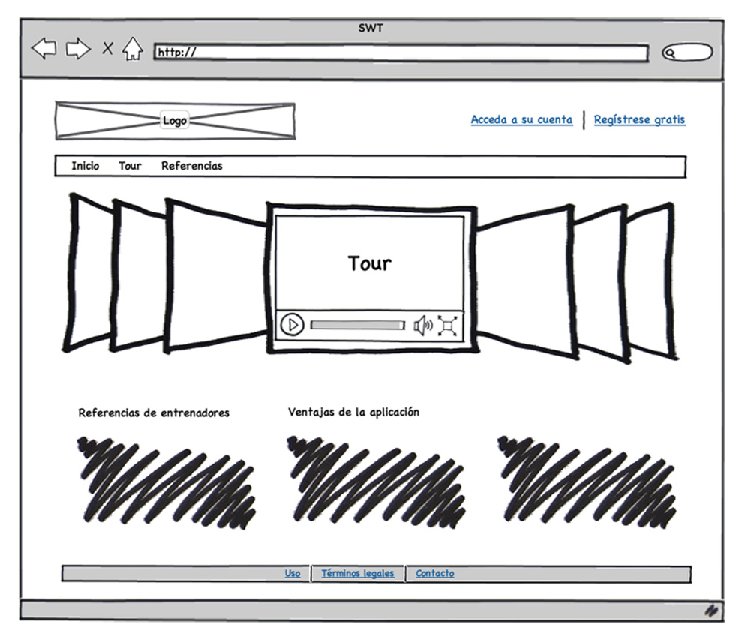
\includegraphics[width=8cm]{./eps/p_interfaz/1_Inicio.eps}
	  \caption{Inicio en la interfaz pública}
	  \label{fig:interfaz_publica_inicio}
	\end{figure}
	
	% subsection introducción (end)
	
	\subsection{Interfaz pública} % (fold)
		\label{sub:interfaz_publica}
		
		La figura \ref{fig:interfaz_publica_inicio} muestra la estructura de la página web que actúa como interfaz pública. La parte superior está compuesta por el logo, enlace a registro/acceso a la aplicación y un menú para acceder al resto de páginas públicas a los entrenadores que aún no estén registrados en el sistema.
			
		El resto de interfaces públicas que la conforman son: {\it tour} con las características y ventajas del sistema (figura \ref{fig:interfaz_publica_tour}); {\it referencias} de los entrenadores que participan en la elaboración del proyecto; página de {\it contacto} (figura \ref{fig:interfaz_publica_contacto}) con los administradores; {\it términos legales y de uso}. 
		
		\begin{figure}[H]
		  \centering
		    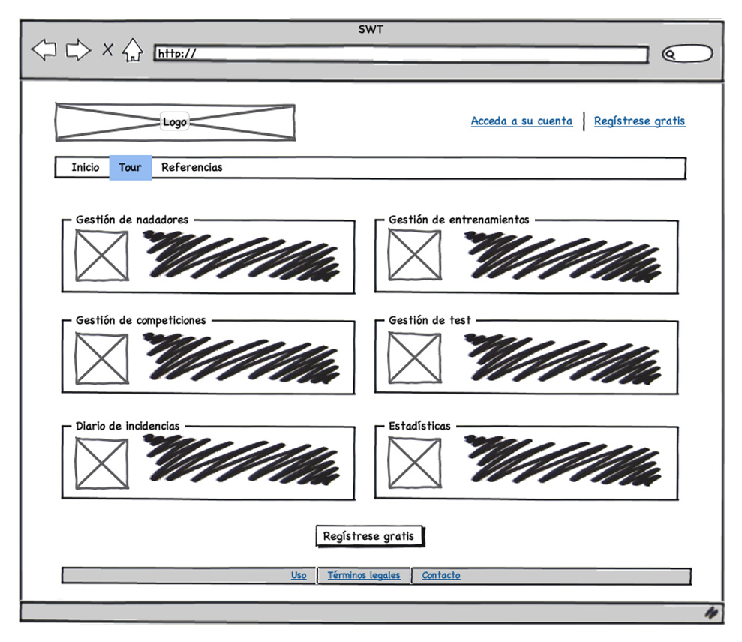
\includegraphics[width=8cm]{./eps/p_interfaz/2_Tour.eps}
		  \caption{Tour en la interfaz pública}
		  \label{fig:interfaz_publica_tour}
		\end{figure}

		\begin{figure}[H]
		  \centering
		    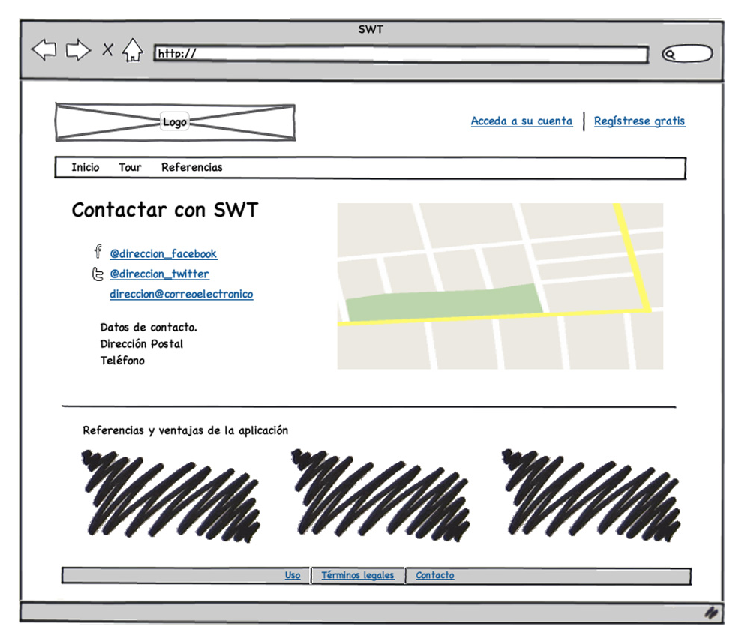
\includegraphics[width=8cm]{./eps/p_interfaz/3_Contacto.eps}
		  \caption{Contacto en la interfaz pública}
		  \label{fig:interfaz_publica_contacto}
		\end{figure}

	% subsection interfaz_pública (end)
	
	\subsection{Registro y acceso} % (fold)
		\label{sub:registro_y_acceso}
	
		Las interfaces para el registro (figura \ref{fig:interfaz_registro}) y acceso (figura \ref{fig:interfaz_acceso}) de un entrenador al sistema son muy similares. Su estructura es algo diferente al resto de páginas de la aplicación, eliminando elementos que puedan interferir en el objetivo último ---registrarse o acceder. Hay que destacar que para el acceso, el identificador de usuario viene proporcionado por el correo electrónico insertado en la fase de registro.
		
		\begin{figure}[H]
		  \centering
		    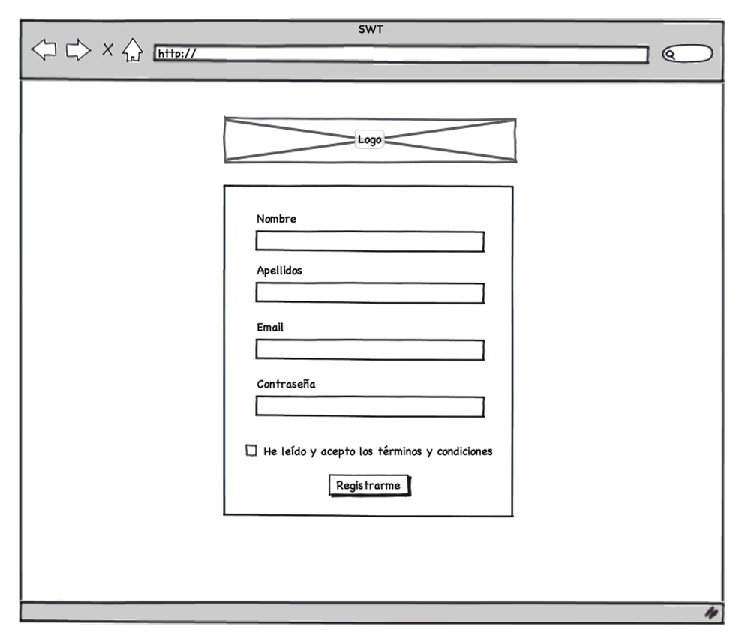
\includegraphics[width=8cm]{./eps/p_interfaz/4_Registro.eps}
		  \caption{Interfaz para el registro de un entrenador}
		  \label{fig:interfaz_registro}
		\end{figure}
		
		\begin{figure}[H]
		  \centering
		    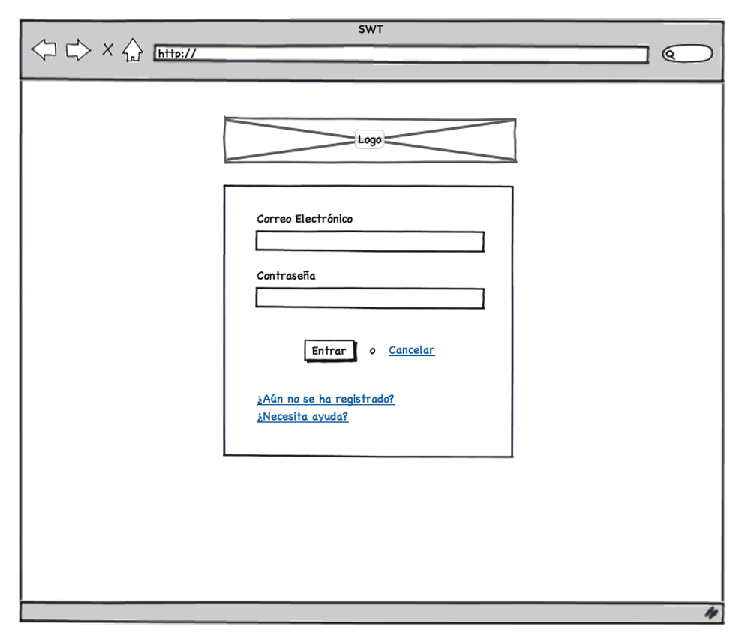
\includegraphics[width=8cm]{./eps/p_interfaz/5_Acceder.eps}
		  \caption{Interfaz para el acceso de un entrenador}
		  \label{fig:interfaz_acceso}
		\end{figure}
	% subsection registro_y_acceso (end)
	
	\subsection{Dashboard} % (fold)
		\label{sub:interfaz_dashboard}
	
	Cuando el entrenador se registra en la aplicación, la primera página a la que accede es la de {\it dashboard} o resumen (figura \ref{fig:interfaz_dashboard}). En ella, lo primero que aparece es un recordatorio de los pasos que tiene que hacer para empezar a sacar provecho de la aplicación. A diferencia de las páginas vistas hasta el momento, ésta incluye en su estructura una barra lateral con los accesos que más frecuentemente se usan.
		
		\begin{figure}[H]
		  \centering
		    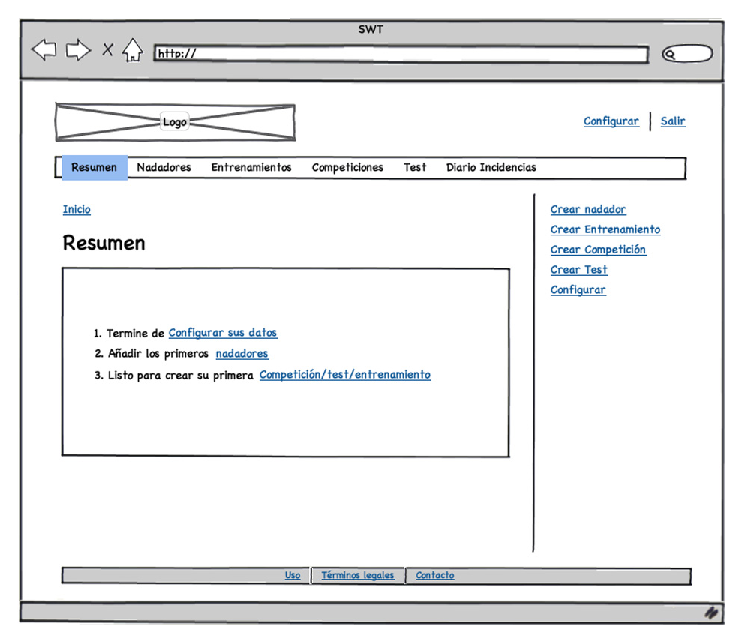
\includegraphics[width=8cm]{./eps/p_interfaz/6_Dashboard.eps}
		  \caption{Interfaz para el dashboard de un entrenador}
		  \label{fig:interfaz_dashboard}
		\end{figure}
		
	% subsection dashboard (end)
	
	\subsection{Configuración del perfil} % (fold)
		\label{sub:configuracion_del_perfil}
	
	Cada entrenador registrado tiene un perfil asociado, donde se guarda información del tipo personal (figura \ref{fig:interfaz_conf_personal}), de contacto (figura \ref{fig:interfaz_conf_contacto}) y los parámetros relacionados con el índice de Mujika (figura \ref{fig:interfaz_conf_mujika}). La información está estructurada en pestañas para una mayor facilidad de navegación.
	
		\begin{figure}[H]
		  \centering
		    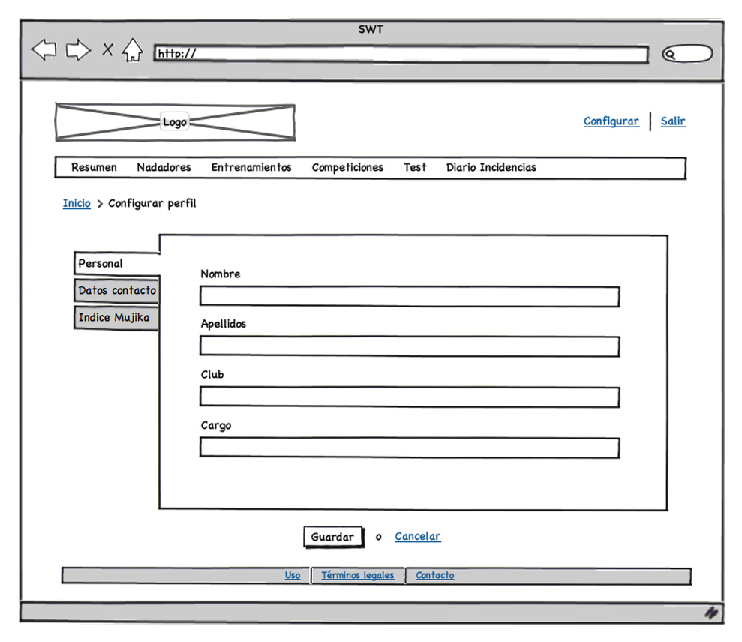
\includegraphics[width=8cm]{./eps/p_interfaz/7_Conf_personal.eps}
		  \caption{Interfaz para la configuración de la información personal en el perfil}
		  \label{fig:interfaz_conf_personal}
		\end{figure}
		
		\begin{figure}[H]
		  \centering
		    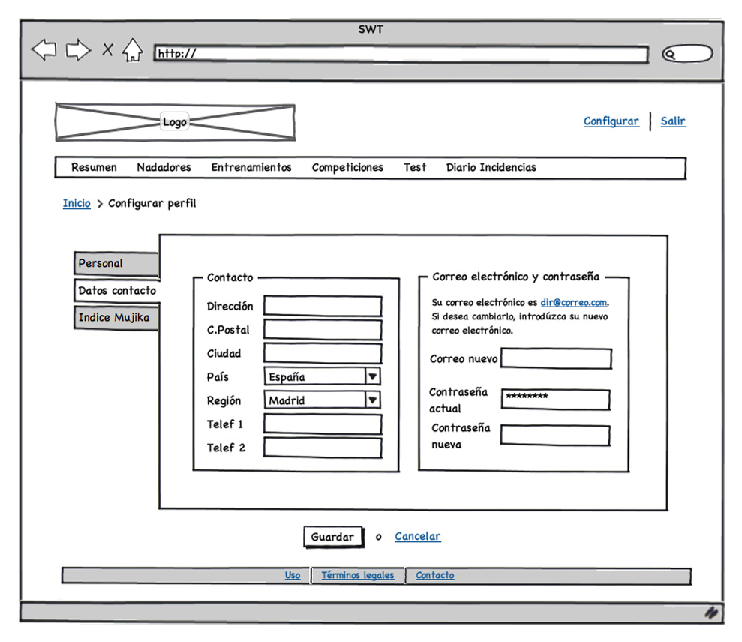
\includegraphics[width=8cm]{./eps/p_interfaz/8_Conf_contacto.eps}
		  \caption{Interfaz para la configuración de la información de contacto en el perfil}
		  \label{fig:interfaz_conf_contacto}
		\end{figure}
		
		\begin{figure}[H]
		  \centering
		    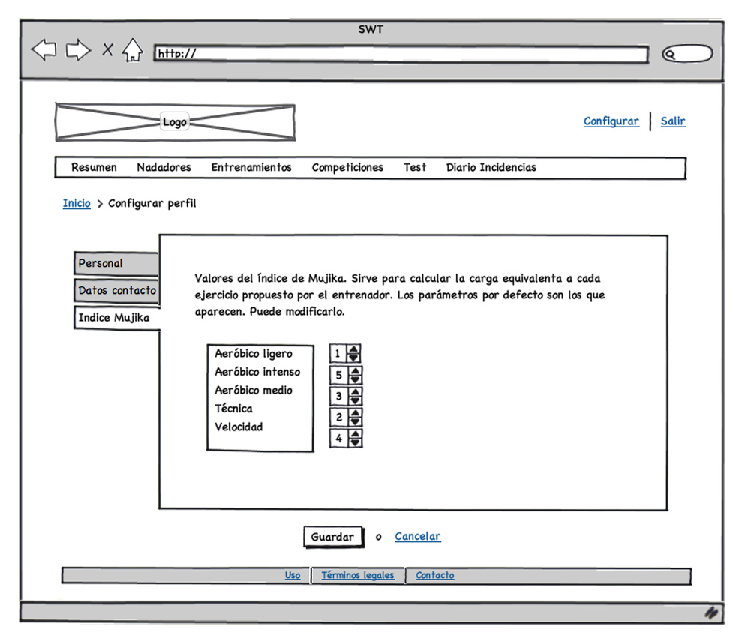
\includegraphics[width=8cm]{./eps/p_interfaz/9_Conf_mujika.eps}
		  \caption{Interfaz para la configuración del índice de Mujika en el perfil}
		  \label{fig:interfaz_conf_mujika}
		\end{figure}
		
	% subsection configuración_del_perfil (end)
	
	\subsection{Gestión de nadadores} % (fold)
		\label{sub:gestion_de_nadadores}
	
	Uno de los módulos fundamentales en la aplicación es el de gestión de nadadores. Es, en gran medida, la base para las competiciones y los test, puesto que los resultados que se insertan en ellos dependen de los nadadores que un entrenador maneja. 
	
	La estructura de la interfaz es común al resto de módulos y está compuesta de:
		
	\begin{itemize}
		\item {{\bf Tabla}. Muestra los registros insertados por un entrenador pertenecientes al módulo en que se encuentre. En este caso, como se está en la sección de nadadores, aparece el conjunto de nadadores que el entrenador ha dado de alta en el sistema.}
		\item {{\bf Buscador}. Campo de búsqueda que localiza registros por diferentes parámetros.}
		\item {{\bf Resumen}. Muestra información relevante al módulo en que se encuentre. Lo normal es que aparezca el número de registros insertados en cada módulo.}
		\item {{\bf Barra lateral}. Desde ella se accede a cada una de las opciones del módulo que se esté gestionando.}
	\end{itemize}
	
	A continuación se muestran las interfaces de {\it ver listado de nadadores} (figura \ref{fig:interfaz_nadadores}), {\it añadir nadador} (figura \ref{fig:interfaz_nadadores_new}), {\it ver nadador} (figura \ref{fig:interfaz_nadadores_show}) y {\it modificar nadador} (figura \ref{fig:interfaz_nadadores_modif}). La primera de ellas muestra todos los nadadores insertados en la aplicación por un entrenador registrado; la segunda refleja el proceso para añadir un nuevo nadador; y la tercera como se modificaría. Es destacable que la información relacionada con las competiciones y test que aparece en {\it ver nadador}, no pueden ser modificadas desde este módulo, sino desde los que gestionan las competiciones y test.
	
	\begin{figure}[H]
	  \centering
	    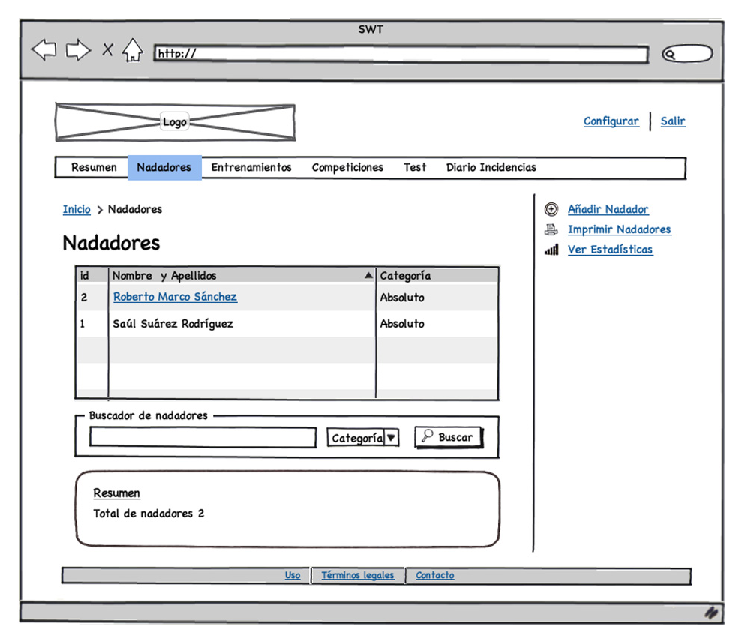
\includegraphics[width=8cm]{./eps/p_interfaz/10_Nadadores.eps}
	  \caption{Interfaz para ver listado de nadadores}
	  \label{fig:interfaz_nadadores}
	\end{figure}
	
	\begin{figure}[H]
	  \centering
	    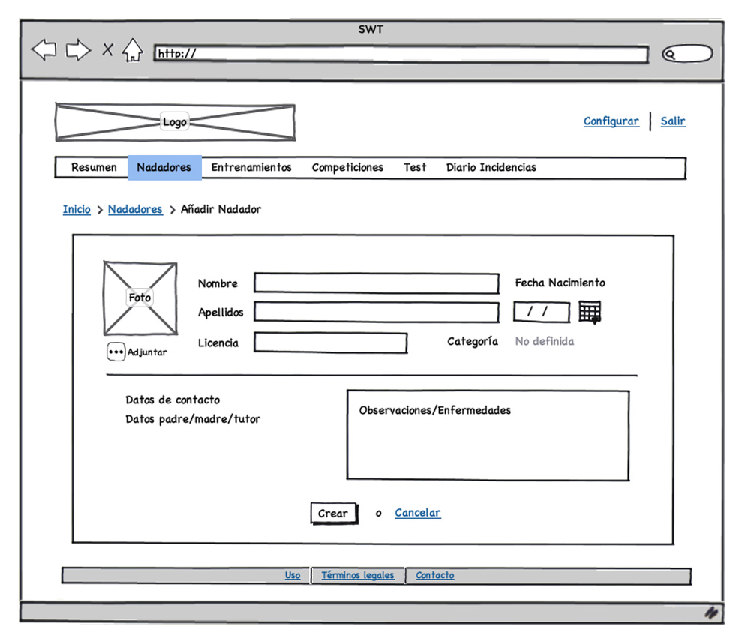
\includegraphics[width=8cm]{./eps/p_interfaz/11_Nadadores_new.eps}
	  \caption{Interfaz para añadir nadador}
	  \label{fig:interfaz_nadadores_new}
	\end{figure}
	
	\begin{figure}[H]
	  \centering
	    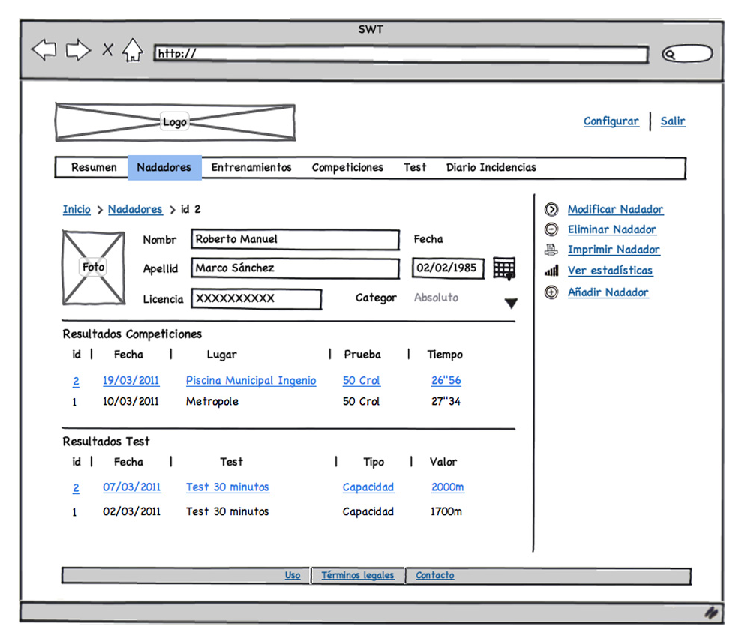
\includegraphics[width=8cm]{./eps/p_interfaz/12_Nadadores_show.eps}
	  \caption{Interfaz para ver nadador}
	  \label{fig:interfaz_nadadores_show}
	\end{figure}
	
	\begin{figure}[H]
	  \centering
	    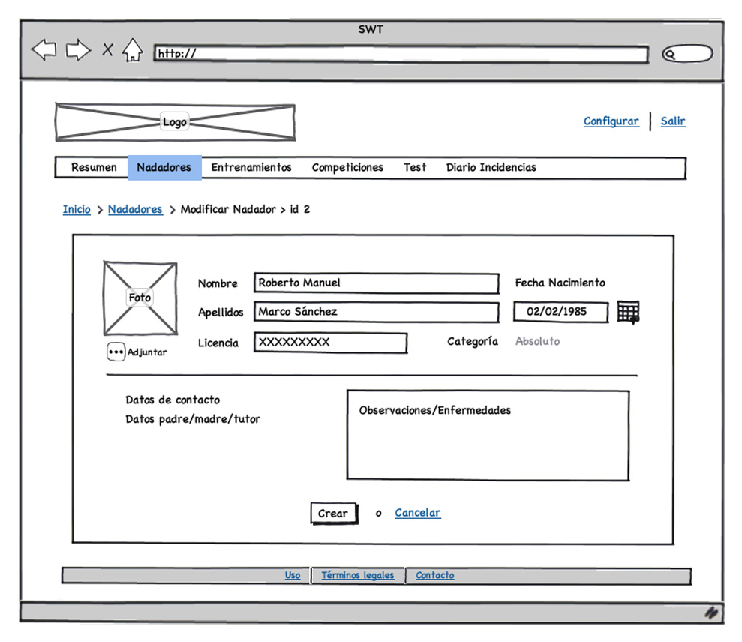
\includegraphics[width=8cm]{./eps/p_interfaz/13_Nadadores_modif.eps}
	  \caption{Interfaz para modificar nadador}
	  \label{fig:interfaz_nadadores_modif}
	\end{figure}
	% subsection gestión_de_nadadores (end)
	
	\subsection{Gestión de Competiciones} % (fold)
		\label{sub:gestion_de_competiciones}
	
	La figura \ref{fig:interfaz_competiciones} muestra la interfaz para ver las competiciones añadidas por un entrenador registrado. Su estructura, como se especificó anteriormente, es similar a la del resto de módulos. La particularidad que tiene es que aparece un calendario de la temporada. A medida que se {\it añadan competiciones} (figura \ref{fig:interfaz_competiciones_new}) irán apareciendo ahí. 
	
		\begin{figure}[H]
		  \centering
		    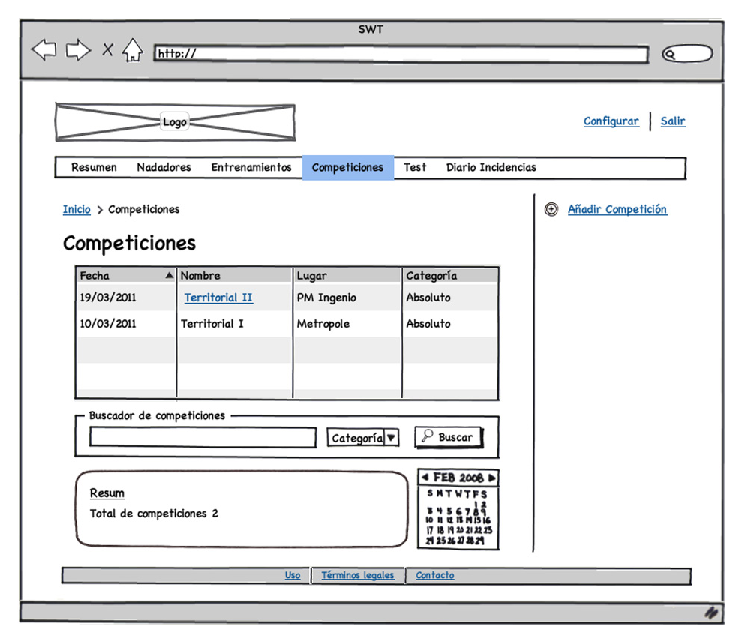
\includegraphics[width=8cm]{./eps/p_interfaz/14_Competiciones.eps}
		  \caption{Interfaz para ver listado de competiciones}
		  \label{fig:interfaz_competiciones}
		\end{figure}

		\begin{figure}[H]
		  \centering
		    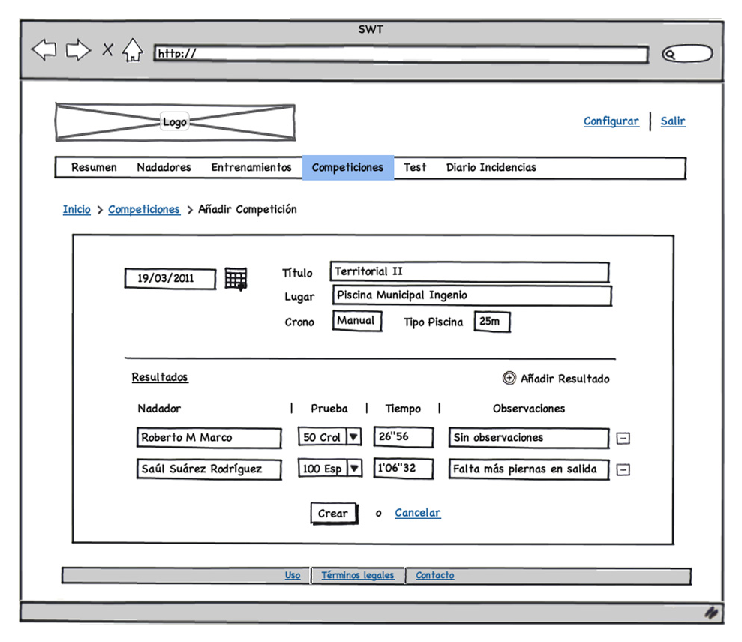
\includegraphics[width=8cm]{./eps/p_interfaz/15_Competiciones_new.eps}
		  \caption{Interfaz para añadir competición}
		  \label{fig:interfaz_competiciones_new}
		\end{figure}

Cuando un entrenador hace clic sobre el nombre de la competición en la tabla, se accede a {\it ver una competición} (figura \ref{fig:interfaz_competiciones_show}). Cuando se modifica una competición (figura \ref{fig:interfaz_competiciones_modif}), se da la posibilidad de modificar cada uno de los resultados añadidos a la misma. Esta información es la que aparecerá modificada en la ficha de cada nadador.

		\begin{figure}[H]
		  \centering
		    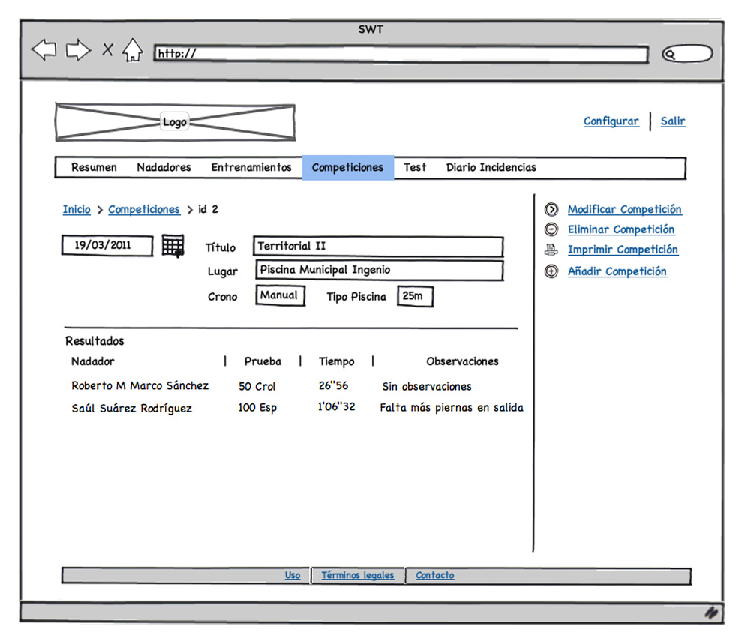
\includegraphics[width=8cm]{./eps/p_interfaz/16_Competiciones_show.eps}
		  \caption{Interfaz para ver competición}
		  \label{fig:interfaz_competiciones_show}
		\end{figure}

		\begin{figure}[H]
		  \centering
		    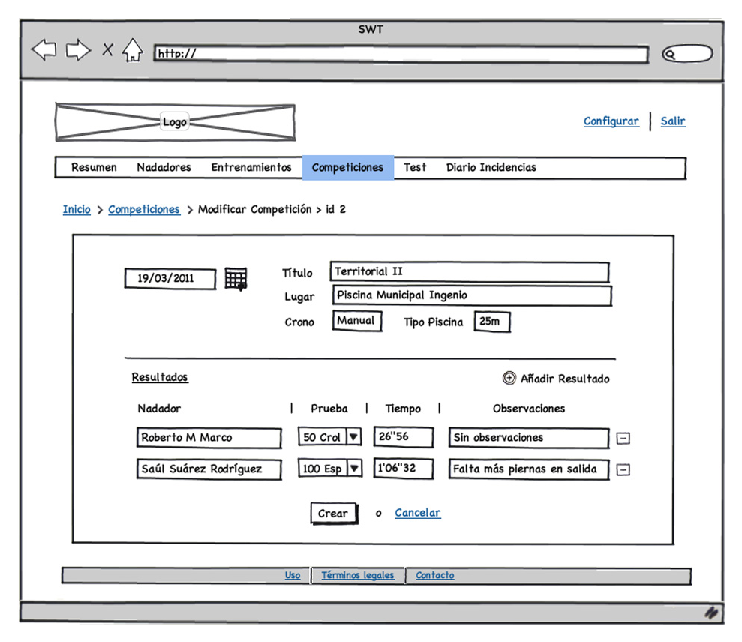
\includegraphics[width=8cm]{./eps/p_interfaz/17_Competiciones_modif.eps}
		  \caption{Interfaz para modificar competición}
		  \label{fig:interfaz_competiciones_modif}
		\end{figure}
	% subsection gestión_de_competiciones (end)
	
	\subsection{Gestión de entrenamientos} % (fold)
		\label{sub:gestion_de_entrenamientos}
	
		\begin{figure}[H]
		  \centering
		    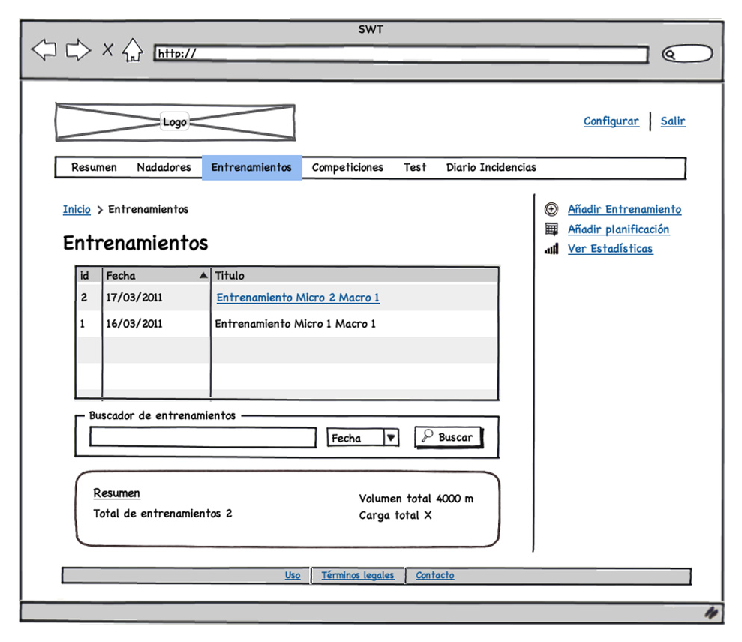
\includegraphics[width=8cm]{./eps/p_interfaz/18_Entrenamientos.eps}
		  \caption{Interfaz para ver listado de entrenamientos}
		  \label{fig:interfaz_entrenamientos}
		\end{figure}
		
	La {\it lista de entrenamientos} (figura \ref{fig:interfaz_entrenamientos}) refleja cada una de las sesiones que inserta el entrenador a lo largo de una temporada. En el resumen se muestran la cantidad de sesiones, el volumen y la carga realizadas en total. Al hacer clic sobre el nombre del entrenamiento, se accede a {\it ver entrenamiento} (figura \ref{fig:interfaz_entrenamientos_show}), que incluye cada uno de los ejercicios añadidos al mismo. Como cada ejercicio tiene asociado un volumen y una carga, se muestra el total de esa sesión. Esto ayuda al entrenador a la hora de hacer los entrenamientos, puesto que conoce el estado a medida que los va desarrollando.\\
	\newline
	{\it Añadir} (figura \ref{fig:interfaz_entrenamientos_new}) y {\it modificar entrenamiento} son iguales, con la salvedad de que el segundo permite cambiar los datos de los formularios que se agregan en el primero.

		\begin{figure}[H]
		  \centering
		    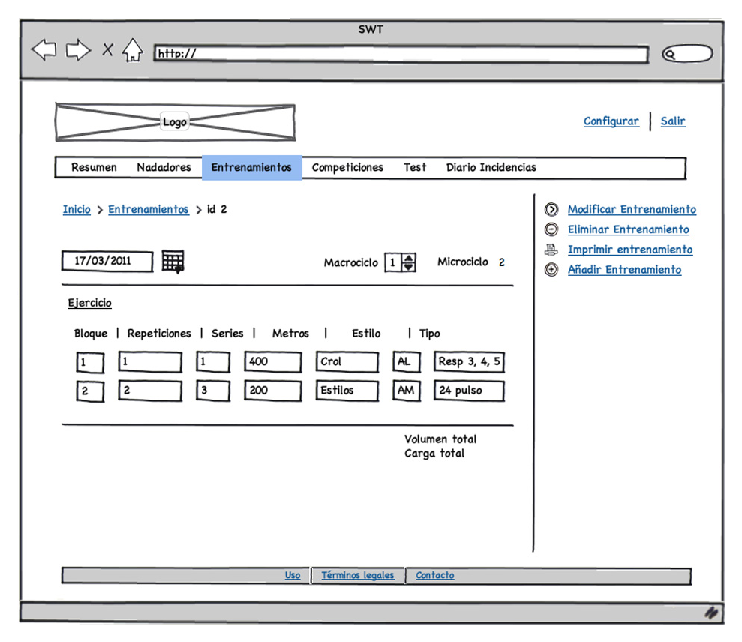
\includegraphics[width=8cm]{./eps/p_interfaz/20_Entrenamientos_show.eps}
		  \caption{Interfaz para ver entrenamiento}
		  \label{fig:interfaz_competiciones_show}
		\end{figure}
	
		\begin{figure}[H]
		  \centering
		    \includegraphics[width=8cm]{./eps/p_interfaz/19_Entrenamientos_new.eps}
		  \caption{Interfaz para añadir entrenamiento}
		  \label{fig:interfaz_entrenamientos_new}
		\end{figure}

	% subsection gestión_de_entrenamientos (end)
	
	\subsection{Gestión de test} % (fold)
		\label{sub:gestion_de_test}
	
	Al igual que para las competiciones, la gestión de test (figura \ref{fig:interfaz_test}) se realiza de la misma forma. La diferencia fundamental está en la información que aparece en la tabla de test insertados por el entrenador en la aplicación. Como para las competiciones, cada uno de los resultados asociados a cada test, aparecen en la ficha de cada nadador.
	
		\begin{figure}[H]
		  \centering
		    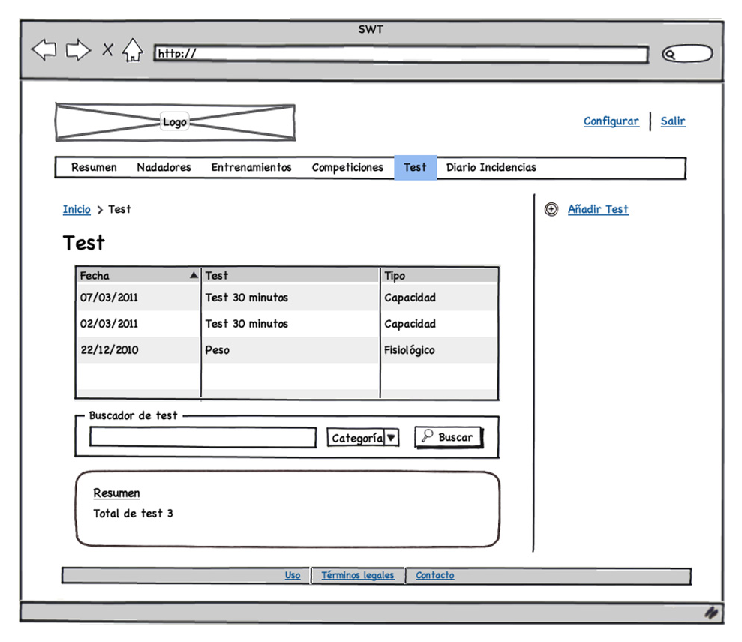
\includegraphics[width=8cm]{./eps/p_interfaz/26_Test.eps}
		  \caption{Interfaz para ver listado de test}
		  \label{fig:interfaz_test}
		\end{figure}
	% subsection gestión_de_test (end)
	
	\subsection{Gestión diario de incidencias} % (fold)
		\label{sub:interfaz_gestion_diario_de_incidencias}
	
	La interfaz para el diario de incidencias del entrenador difiere del resto en que, cada incidencia, tiene asociada una o varias etiquetas. Por ello, en el resumen que aparece en la interfaz de {\it ver diario de incidencias} (figura \ref{fig:interfaz_incidencias}), se muestran los valores más usados por los entrenadores. Esto ayudará a localizar rápidamente cada tipo de incidencia. Como en casos anteriores, a continuación se muestra {\it ver incidencia} (figura \ref{fig:interfaz_incidencias_show}), {\it añadir incidencia} (figura \ref{fig:interfaz_incidencias_new}) y {\it modificar incidencia} (figura \ref{fig:interfaz_incidencias_modif}).
	
		\begin{figure}[H]
		  \centering
		    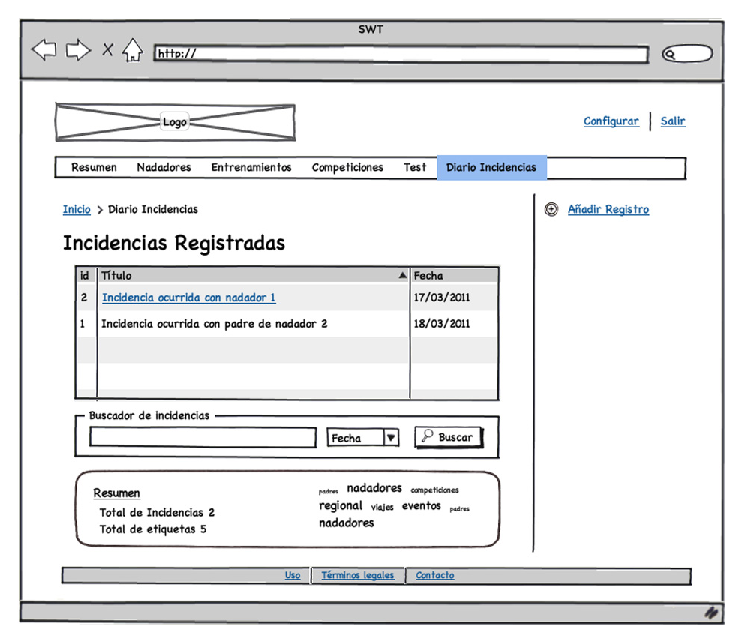
\includegraphics[width=8cm]{./eps/p_interfaz/22_Diario.eps}
		  \caption{Interfaz para ver diario de incidencias}
		  \label{fig:interfaz_incidencias}
		\end{figure}

		\begin{figure}[H]
		  \centering
		    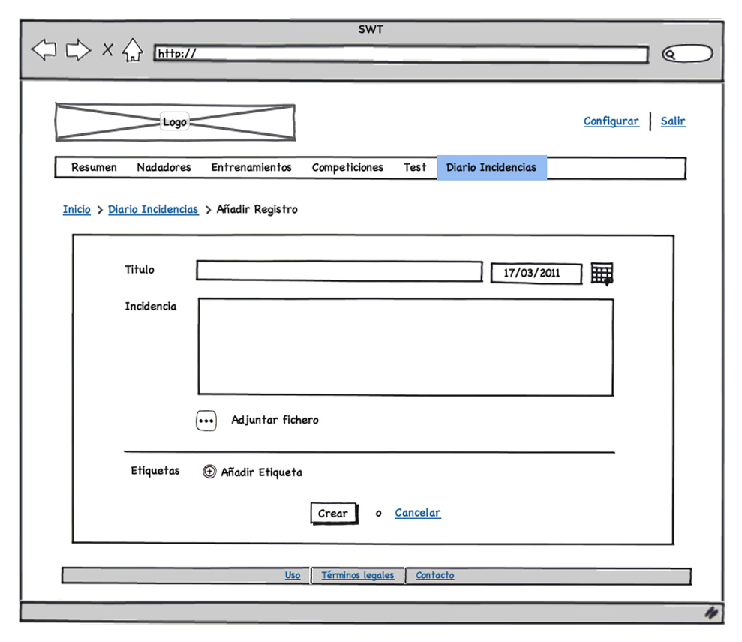
\includegraphics[width=8cm]{./eps/p_interfaz/23_Diario_new.eps}
		  \caption{Interfaz para añadir incidencia}
		  \label{fig:interfaz_incidencias_new}
		\end{figure}
		
		\begin{figure}[H]
		  \centering
		    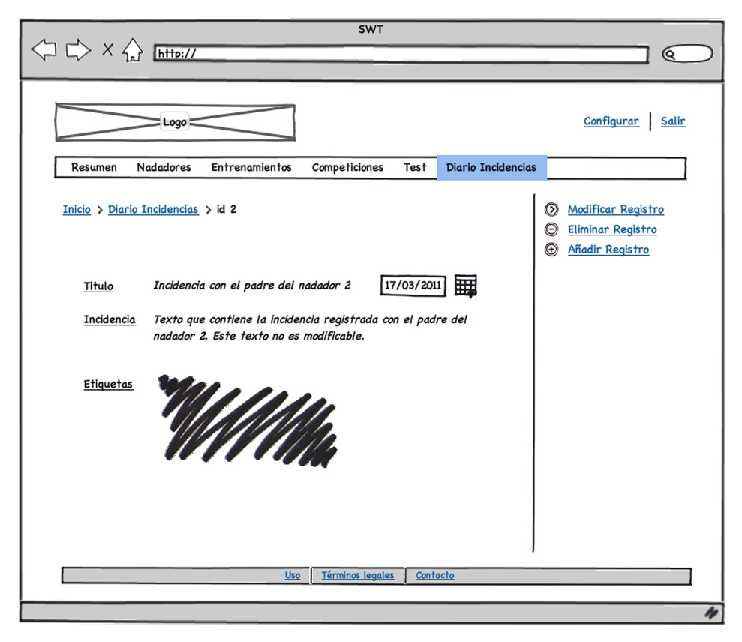
\includegraphics[width=8cm]{./eps/p_interfaz/24_Diario_show.eps}
		  \caption{Interfaz para ver incidencia}
		  \label{fig:interfaz_incidencias_show}
		\end{figure}

		\begin{figure}[H]
		  \centering
		    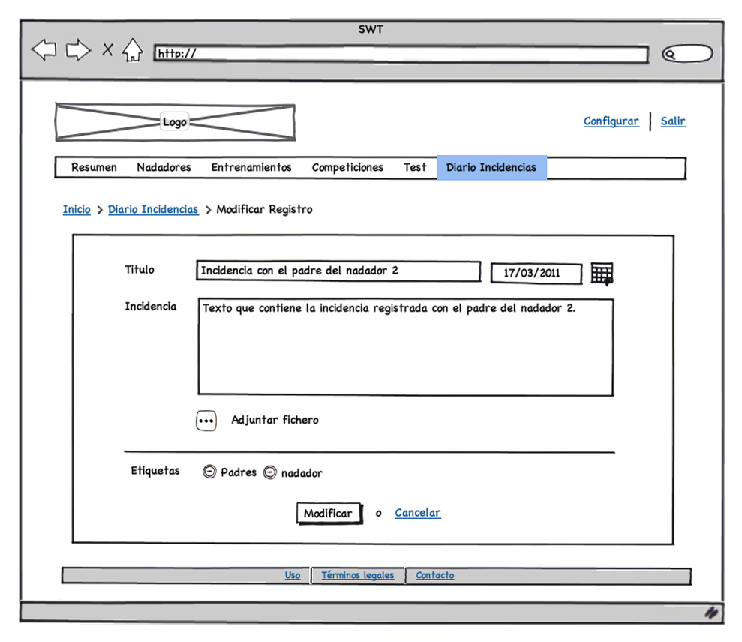
\includegraphics[width=8cm]{./eps/p_interfaz/25_Diario_modif.eps}
		  \caption{Interfaz para modificar incidencia}
		  \label{fig:interfaz_incidencias_modif}
		\end{figure}
	% subsection interfaz_gestión_diario_de_incidencias (end)
% section diseño_de_interfaz_de_usuario (end)
% chapter análisis (end)